\chapter{Methodology}
\label{ch:method}

This chapter details the methodology employed to analyze and optimize the transportation network for students of the Izmir Institute of Technology residing in Izmir. The primary objective is to identify efficient bus routing strategies that minimize overall fuel consumption while adhering to practical constraints on bus capacity. Specifically, the network serves approximately 2000 students, and routes must accommodate a minimum of 10 and a maximum of 50 students per vehicle. 

Our approach leverages graph theory, treating student locations as nodes and potential travel segments as edges. We systematically explore various graph construction techniques and clustering algorithms to model the spatial relationships and identify optimal bus routes. The methodology is divided into three main sections: graph representation of the transportation map, clustering of the graph representations, and robustness analysis for the clustering solutions.

\section{Graph Representation of Transportation Map of IZTECH}
\label{sec:graph_representation}

The foundation of our analysis is a dataset comprising the geographical coordinates of approximately 2000 synthetically generated student locations throughout Izmir. These points were created by applying a Gaussian distribution based on the actual population data for each district in Izmir. Figure \ref{fig:student_map} illustrates the geographical distribution of these student locations. In our graph-based model, each student's location is represented as a distinct node (or vertex) $v$ within a set $V$. The set $V$ thus encapsulates all student locations considered in the transportation network, where $|V| \approx 2000$. 

% Placeholder for Map Visualization
\begin{figure}[!htbp]
\centering
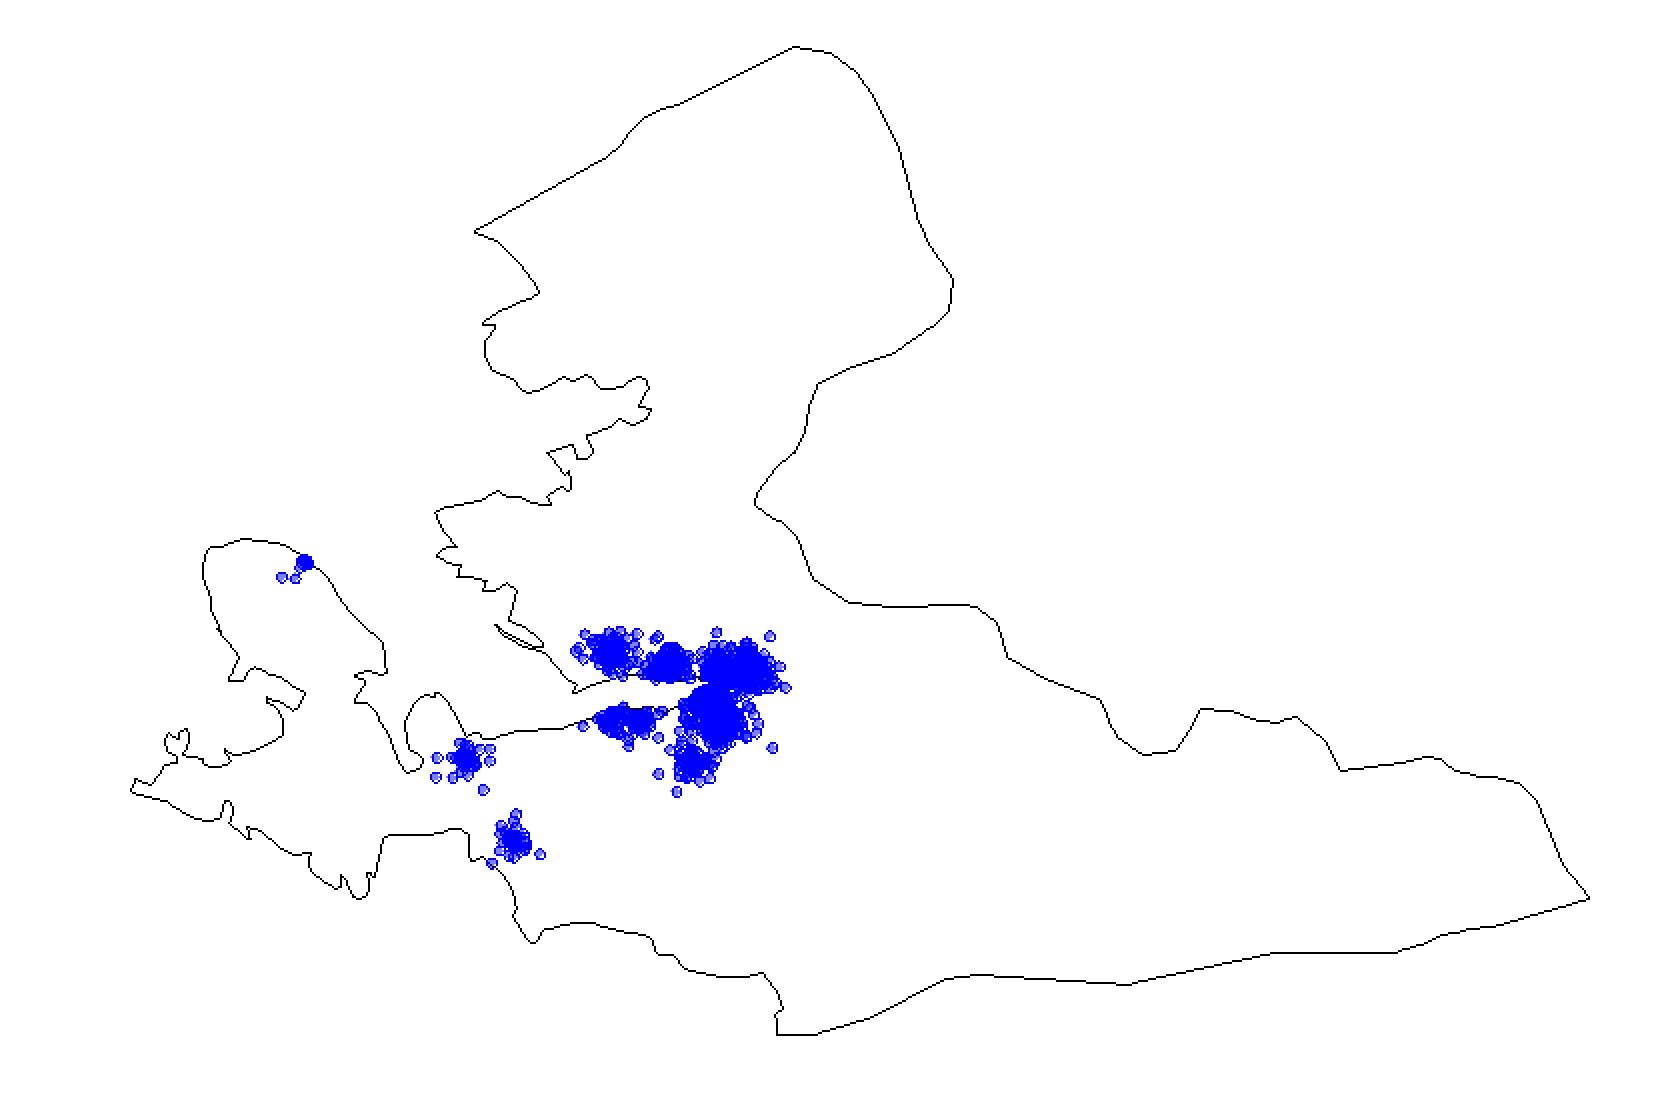
\includegraphics[width=0.8\textwidth]{img/student_map}
\caption{Geographical distribution of student locations in Izmir.}
\label{fig:student_map}
\end{figure}

\subsection{Complete Graph Representation}
\label{subsec:complete_graph}

A complete graph is the natural mathematical representation of a transportation network where every location is directly connected to every other location. Formally, for our set of student locations $V$, the complete graph $G_{complete} = (V, E_{complete})$ contains an edge $e_{uv} \in E_{complete}$ for every pair of distinct vertices $u, v \in V$, resulting in $|E_{complete}| = {|V| \choose 2} = \frac{|V|(|V|-1)}{2}$ edges. The complete graph connects every pair of distinct student locations, representing maximum potential connectivity as detailed in Section~\ref{se:GraphConstructionMethodsAndSparsity}.

This representation serves as our baseline model, establishing upper bounds on connectivity. However, the dense connectivity often leads to suboptimal routing solutions with higher overall costs due to the ${|V| \choose 2}$ edges making it computationally expensive for large datasets.

\begin{figure}[!htbp]
\centering
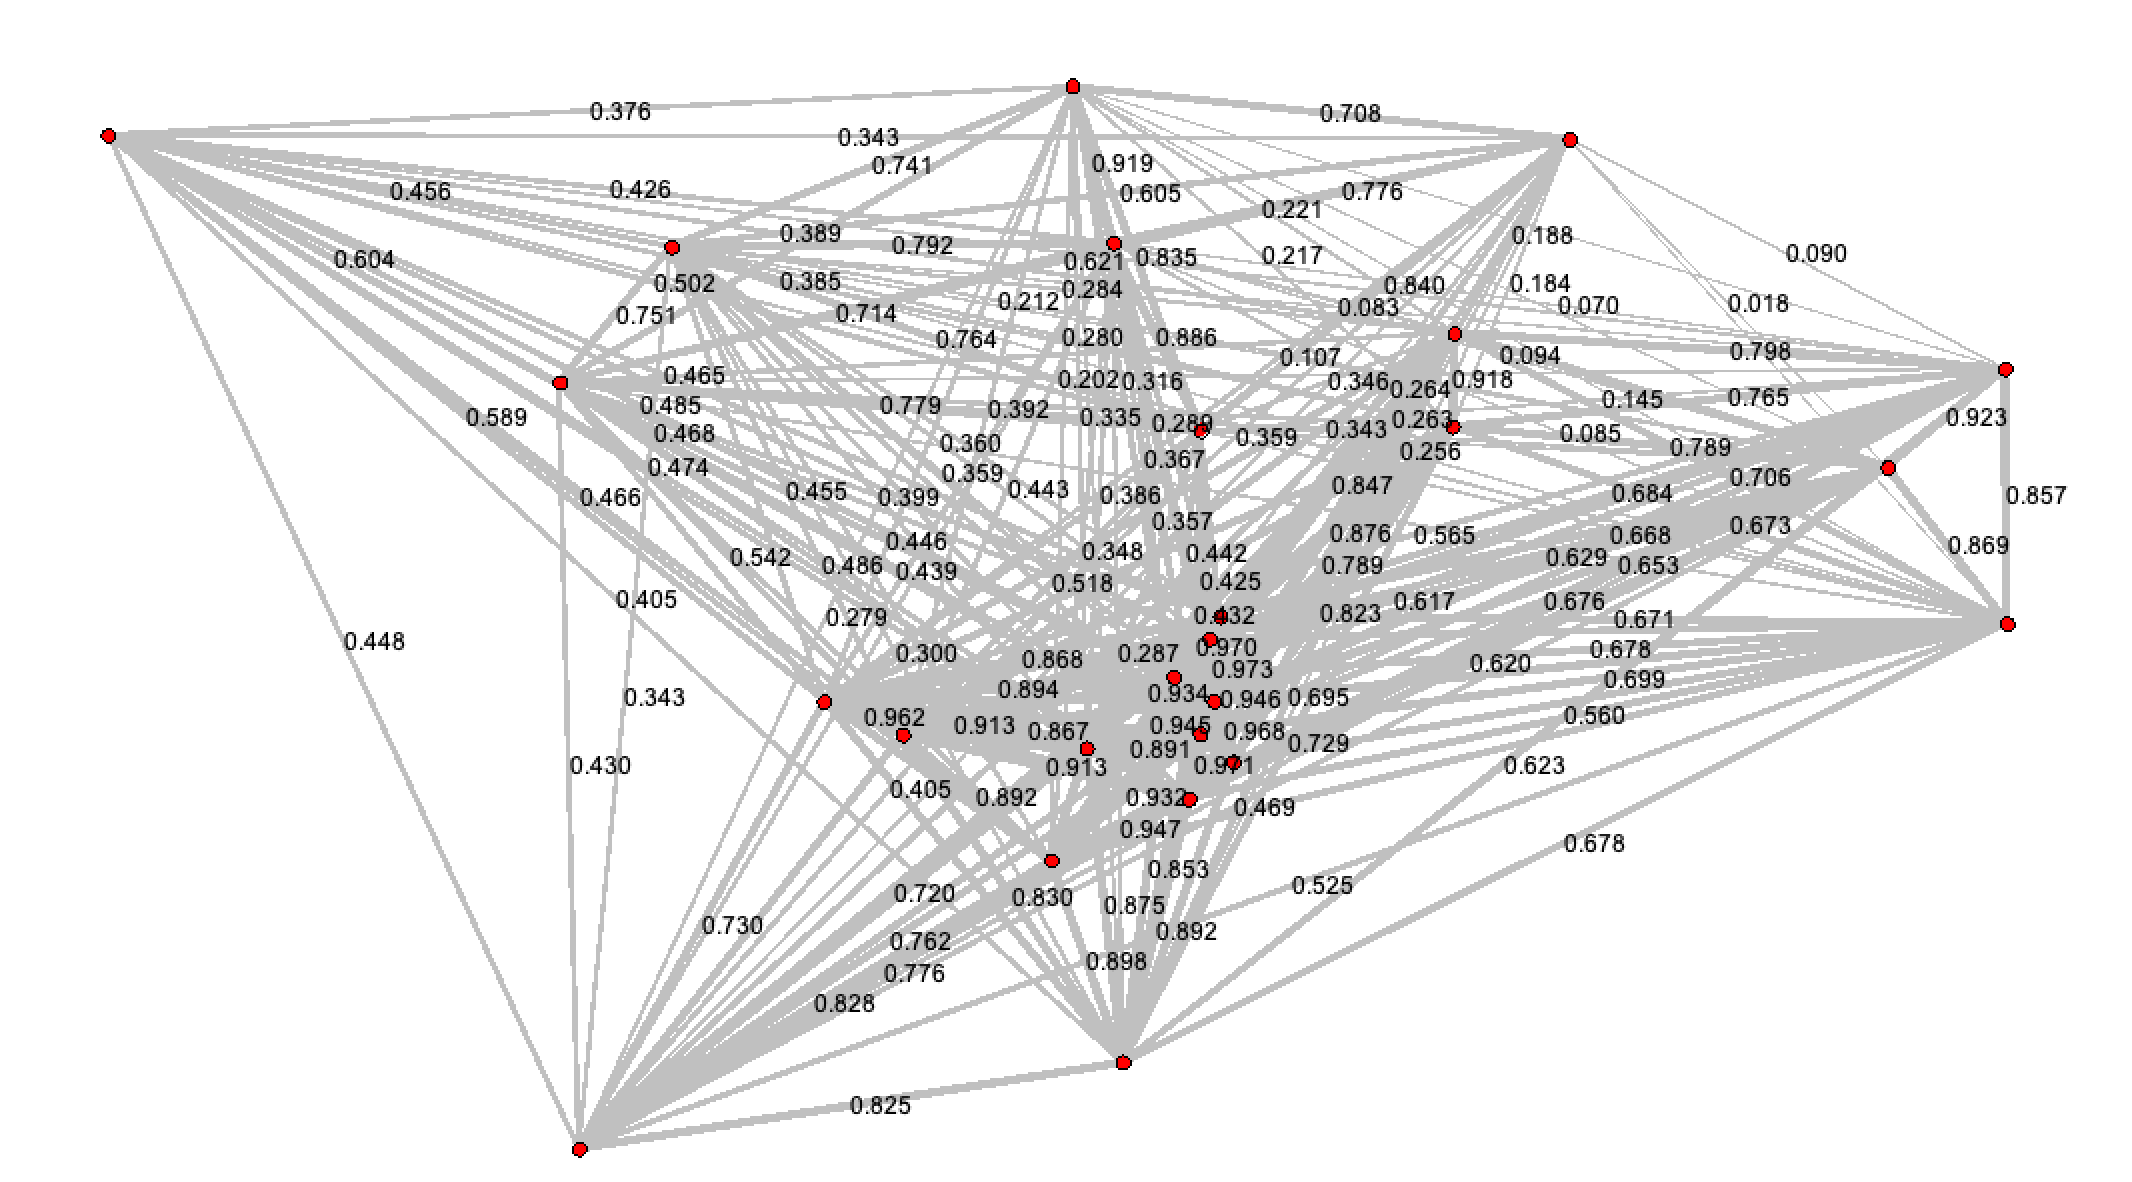
\includegraphics[width=0.6\textwidth]{img/complete}
\caption{Complete graph representation of a sample of student locations. Every point is connected to every other point, representing maximum connectivity but leading to computational challenges for large datasets.}
\label{fig:complete_graph}
\end{figure}



\subsection{Sparse Graph Representation}
\label{subsec:sparse_graph}

Given the computational and practical limitations of the complete graph approach, we explored several sparse graph construction techniques that preserve essential connectivity while significantly reducing the number of edges. These methods emphasize local connections and spatial proximity, resulting in more efficient representations of the transportation network.

\subsubsection{Delaunay Graph Representation}
\label{subsubsec:delaunay}

The Delaunay triangulation constructs a graph $G_{Delaunay}=(V, E_{Delaunay})$ based on the empty circumcircle property as explained in Section~\ref{se:GraphConstructionMethodsAndSparsity}. For any three vertices $p, q, r \in V$, they form a triangle in the Delaunay triangulation if and only if the circumcircle passing through $p, q, r$ contains no other vertex in $V$. This property creates a planar graph that avoids edge crossings and naturally connects proximate points.

\begin{figure}[!htbp]
\centering
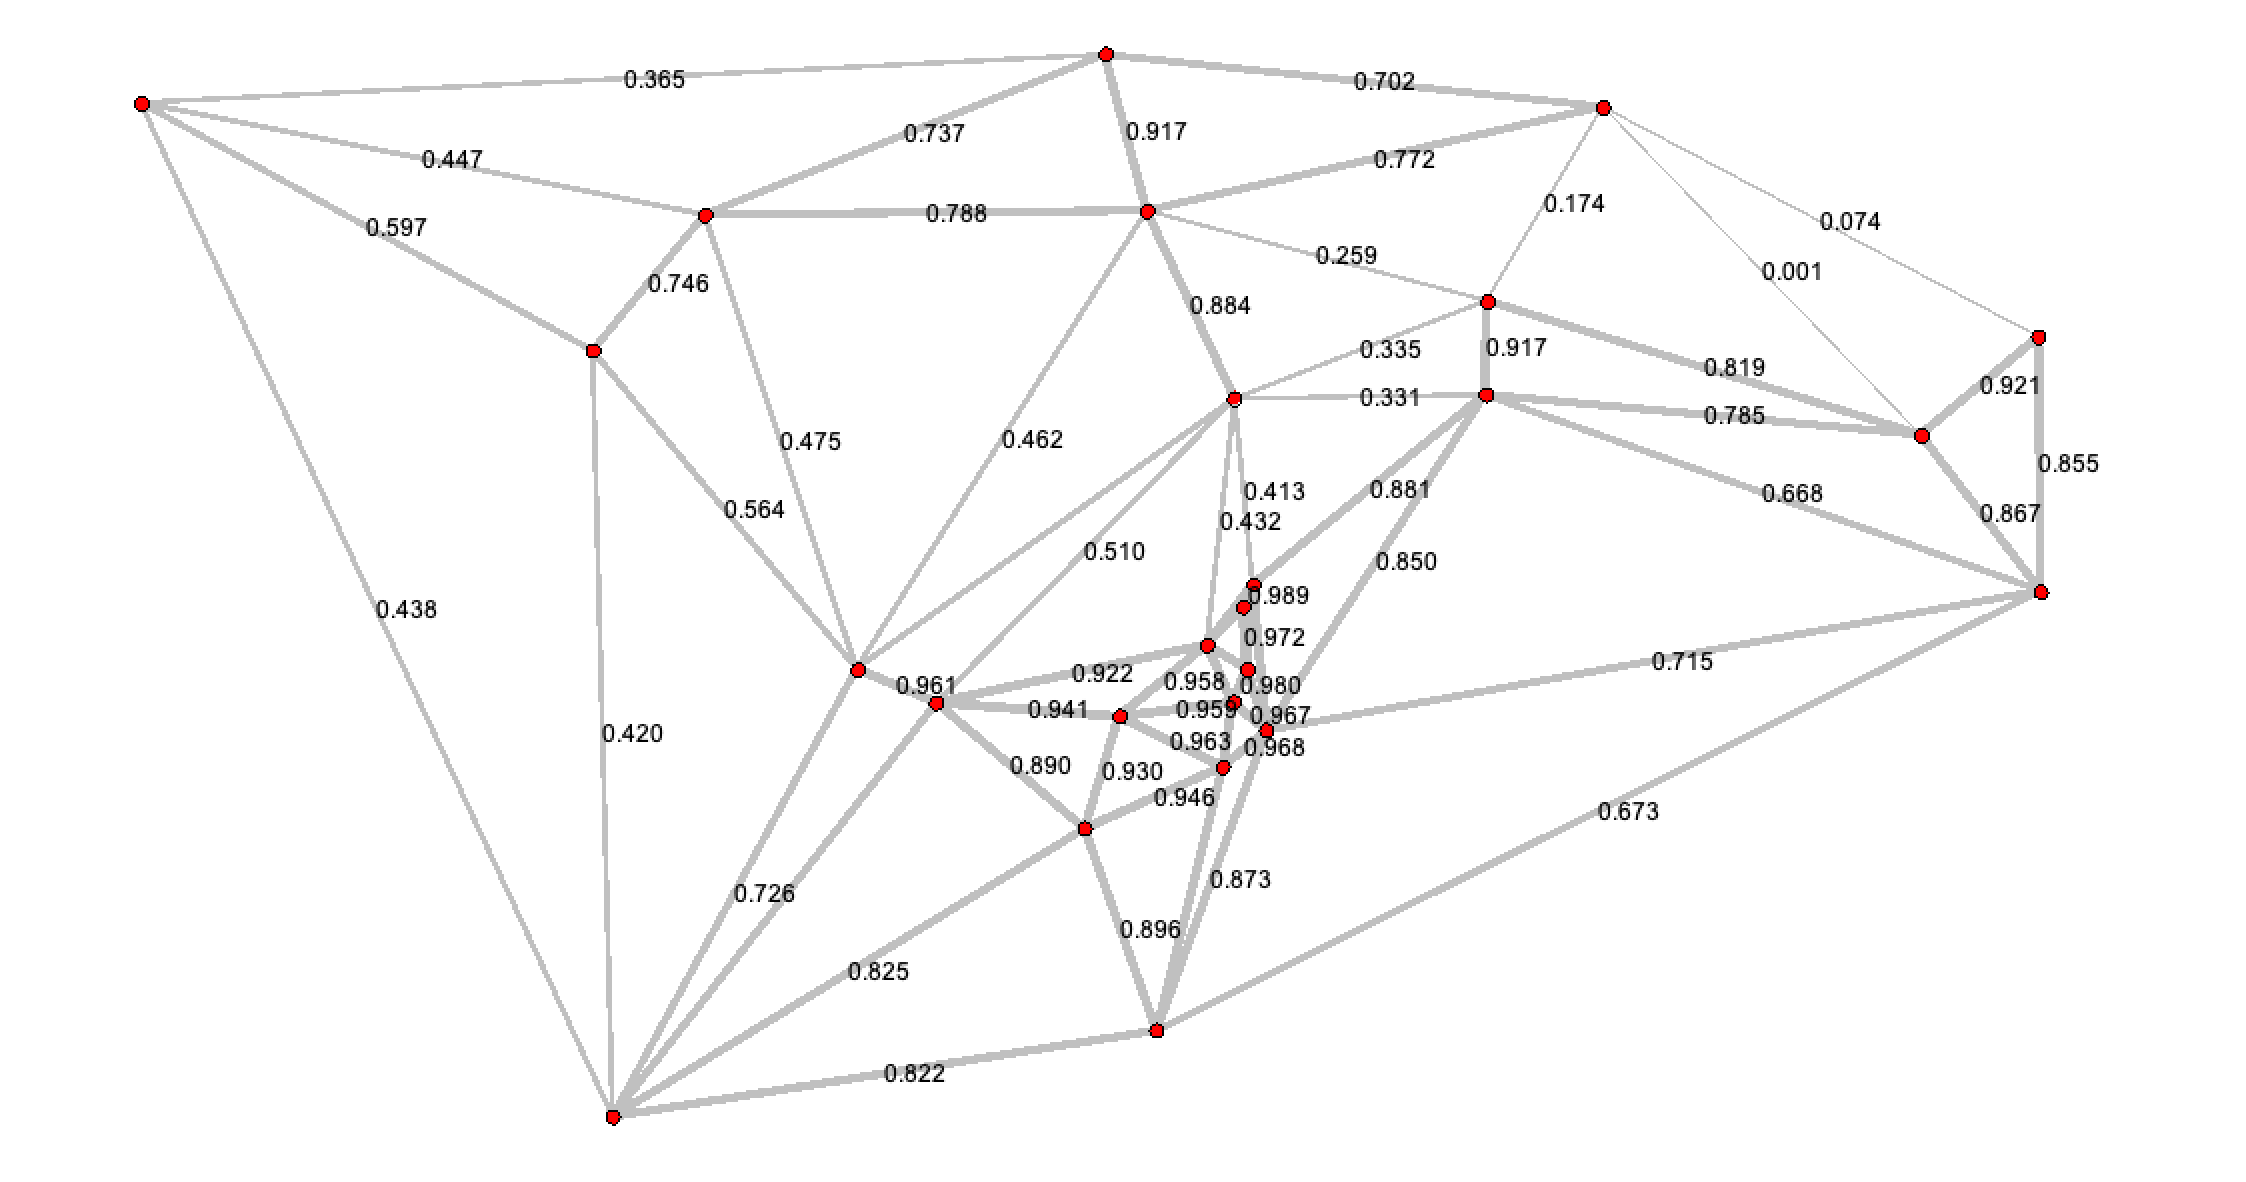
\includegraphics[width=0.6\textwidth]{img/delaunay}
\caption{Delaunay triangulation applied to a sample of student locations. The triangulation connects points such that no point lies inside the circumcircle of any triangle, creating a network that naturally preserves proximity relationships.}
\label{fig:delaunay_graph}
\end{figure}

\subsubsection{Gabriel Graph Representation}
\label{subsubsec:gabriel}

The Gabriel graph is a subgraph of the Delaunay triangulation that connects nodes if the circle with diameter between them contains no other nodes (see Section~\ref{se:GraphConstructionMethodsAndSparsity}). Formally, for our set of student locations $V$, the Gabriel graph $G_{Gabriel}=(V, E_{Gabriel})$ contains an edge $e_{uv} \in E_{Gabriel}$ if and only if:

\begin{equation}
d^2(u, v) < d^2(u, w) + d^2(v, w) \text{ for all } w \in V, w \neq u, w \neq v
\end{equation}

where $d(u, v)$ represents the Euclidean distance between vertices $u$ and $v$.

Our implementation constructs the Gabriel graph by first generating the Delaunay triangulation and then filtering edges based on the empty circle criterion. This approach preserves the most efficient local connections while further reducing the computational complexity compared to the complete graph.

\begin{figure}[!htbp]
\centering
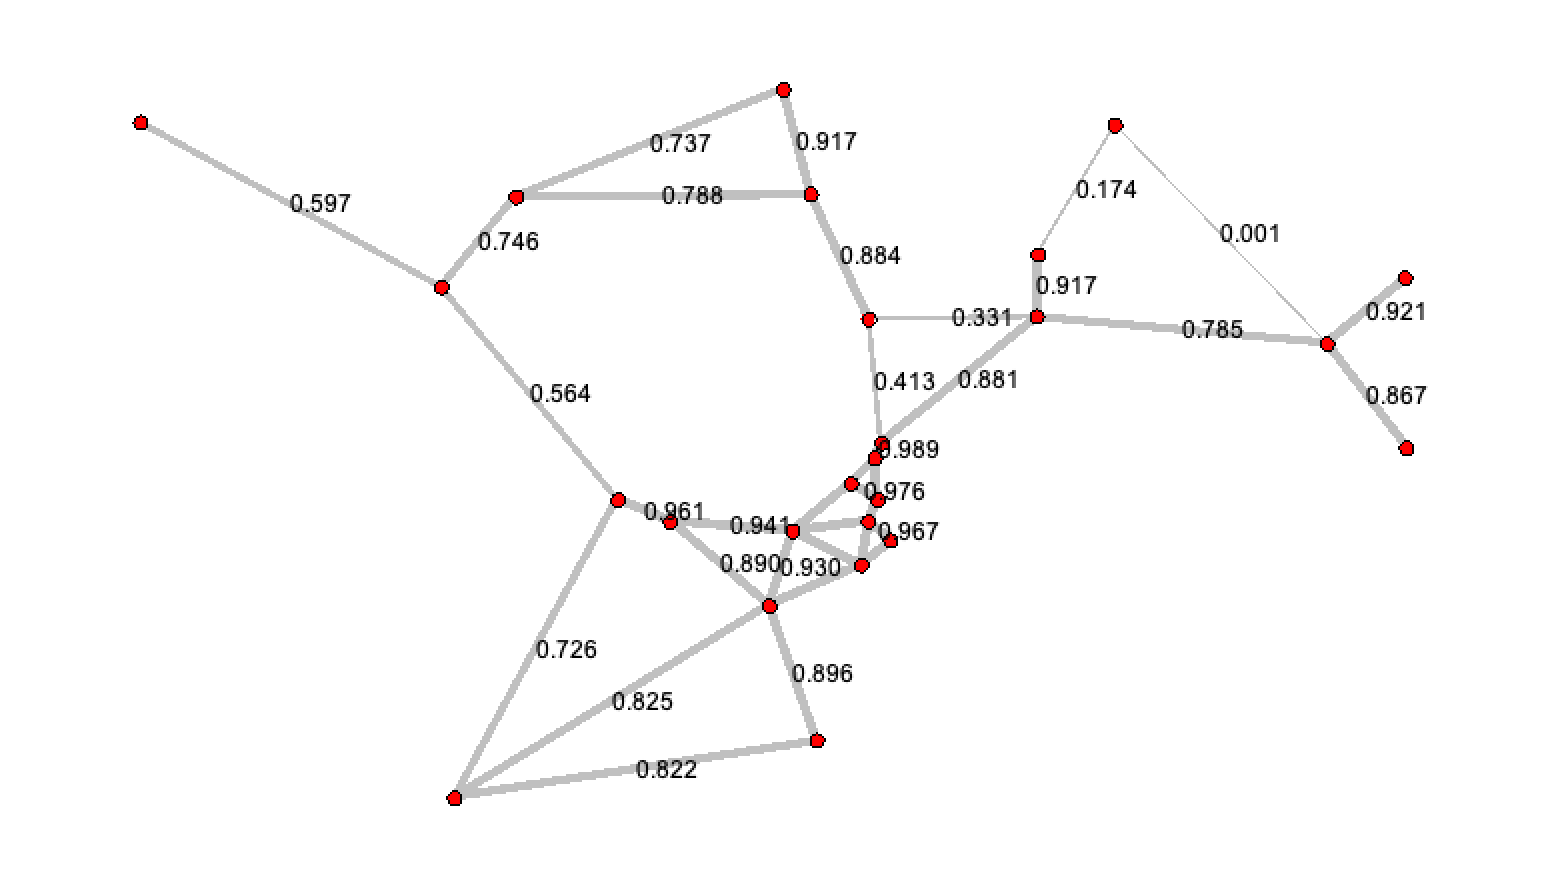
\includegraphics[width=0.6\textwidth]{img/gabriel}
\caption{Gabriel graph derived from student location data. This graph is a subgraph of the Delaunay triangulation, where an edge between two points exists only if the circle with the diameter equal to the distance between them contains no other points.}
\label{fig:gabriel_graph}
\end{figure}

\subsubsection{K-Nearest Neighbour Graph Representation}
\label{subsubsec:knn}

The K-Nearest Neighbors (KNN) graph connects each node to its $k$ closest neighbors, creating a sparse representation that emphasizes local connectivity as detailed in Section~\ref{se:GraphConstructionMethodsAndSparsity}. For our set of student locations $V$, the KNN graph $G_{KNN}=(V, E_{KNN})$ contains edges such that:

\begin{equation}
E_{KNN} = \{(u, v) \mid v \in \text{kNN}(u) \text{ or } u \in \text{kNN}(v)\}
\end{equation}

where $\text{kNN}(u)$ represents the $k$ nearest neighbors of vertex $u$ according to Euclidean distance.

In our implementation, we set $k=30$ based on the average seat size of buses in the IZTECH fleet, ensuring that each node is connected to approximately the number of students that would typically share transportation. The graph is constructed using spatial indexing for efficient neighbor queries, with edge weights based on the Euclidean distance between connected nodes.

\begin{figure}[!htbp]
\centering
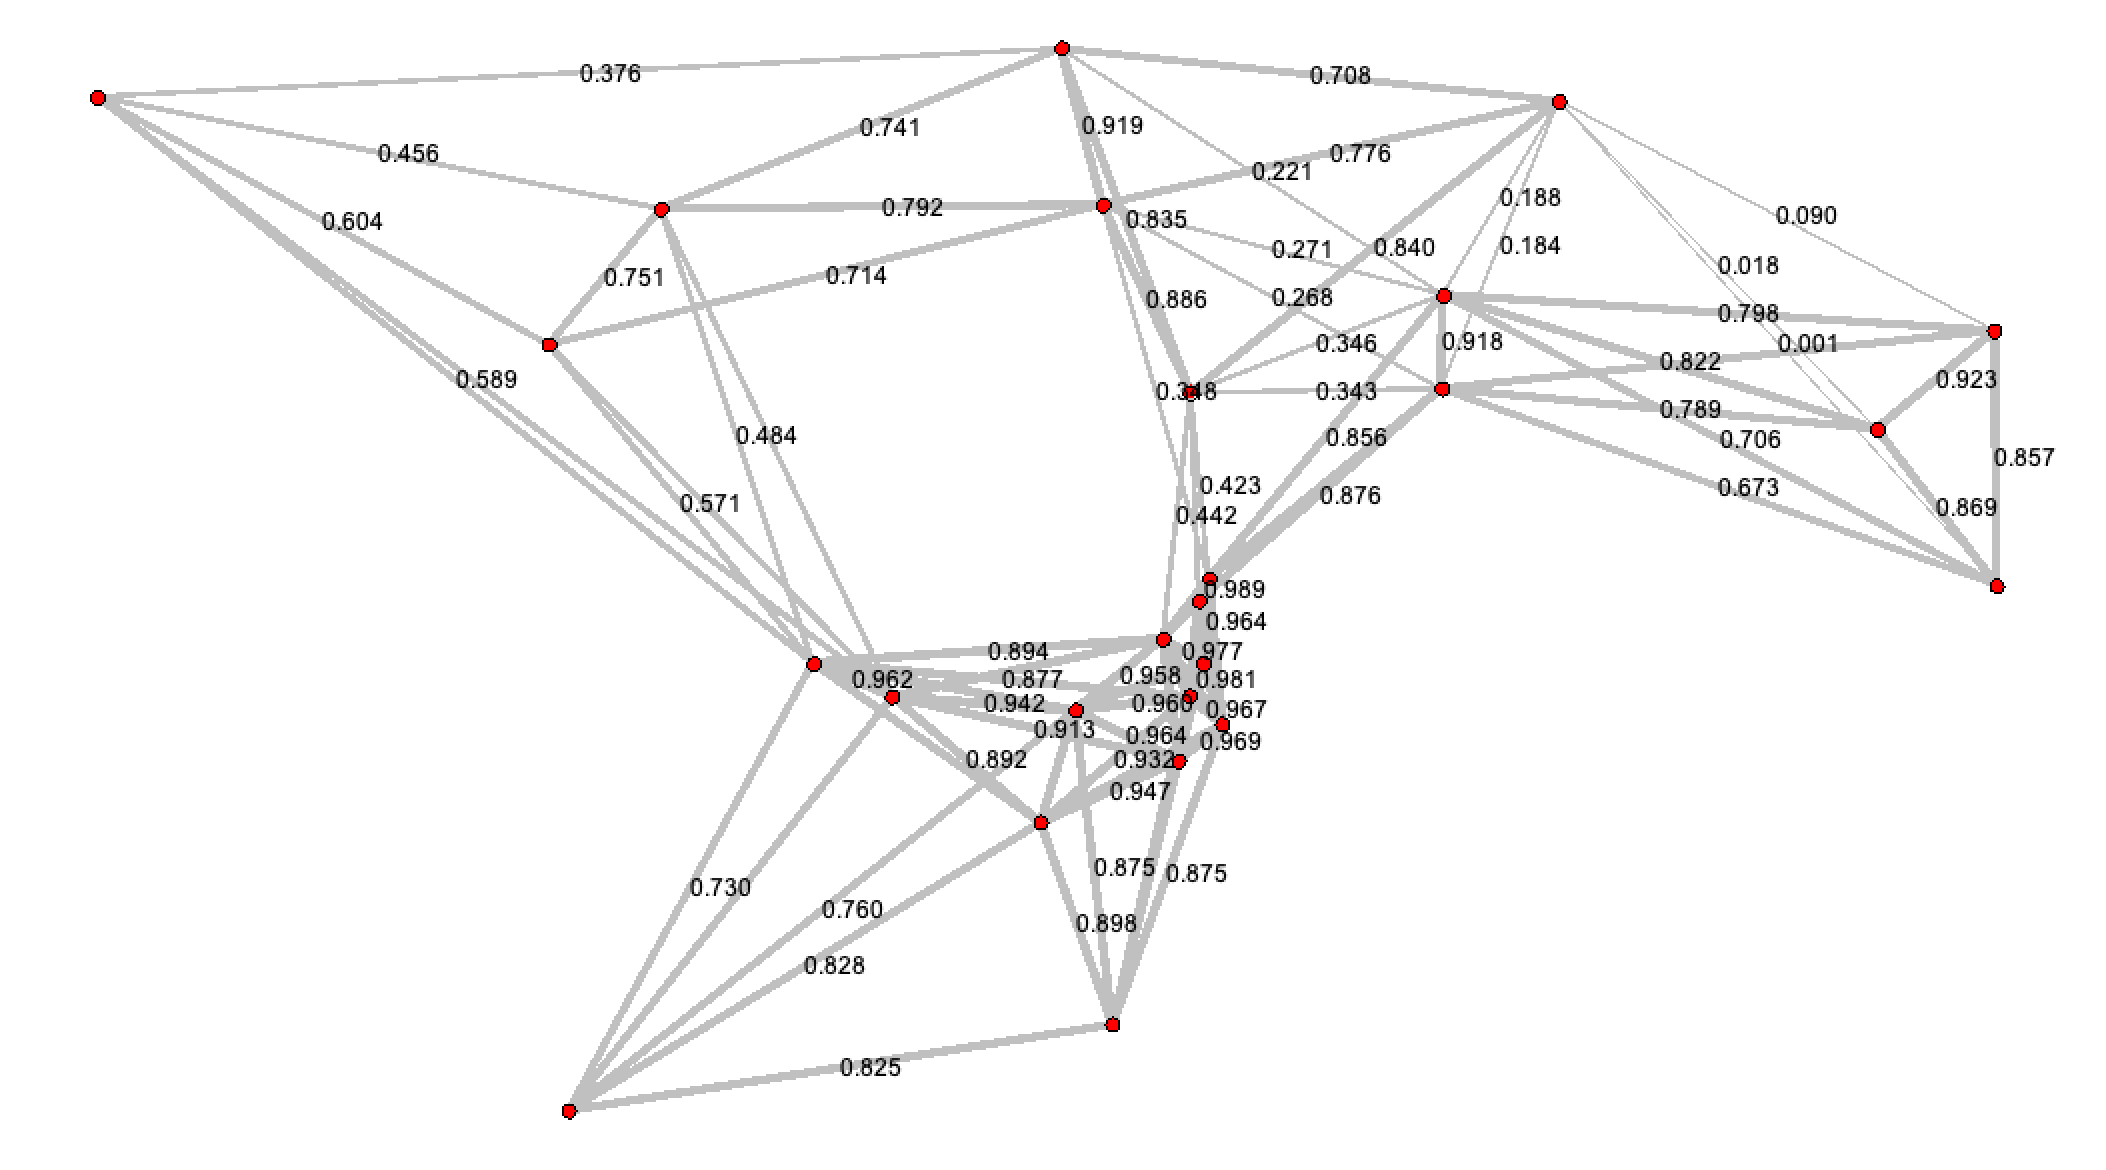
\includegraphics[width=0.6\textwidth]{img/k_nearest}
\caption{K-Nearest Neighbors graph with $k=5$ applied to student location data. Each point is connected to its five closest neighbors, creating a sparse network that preserves local connectivity while significantly reducing the number of edges compared to the complete graph.}
\label{fig:knn_graph}
\end{figure}

\section{Clustering Graph Representationof Transportation Map of IZTECH}
\label{sec:clustering_graph}

Once the various graph representations were constructed, we applied clustering algorithms to partition the nodes (students) into clusters, representing potential bus routes. The clustering phase is critical for identifying cohesive groups of students who can be efficiently transported together.

\subsection{Clustering Complete Graph Representation}
\label{subsec:clustering_complete}

Clustering the complete graph representation presents unique challenges due to its dense connectivity. Our implementation applies multiple clustering algorithms to the complete graph, each configured to respect the bus capacity constraints. We enforced a minimum cluster size of 10 students (minimum efficient bus occupancy) and a maximum cluster size of 50 students (maximum bus capacity) to ensure practical viability of the resulting routes.

\begin{figure}[!htbp]
\centering
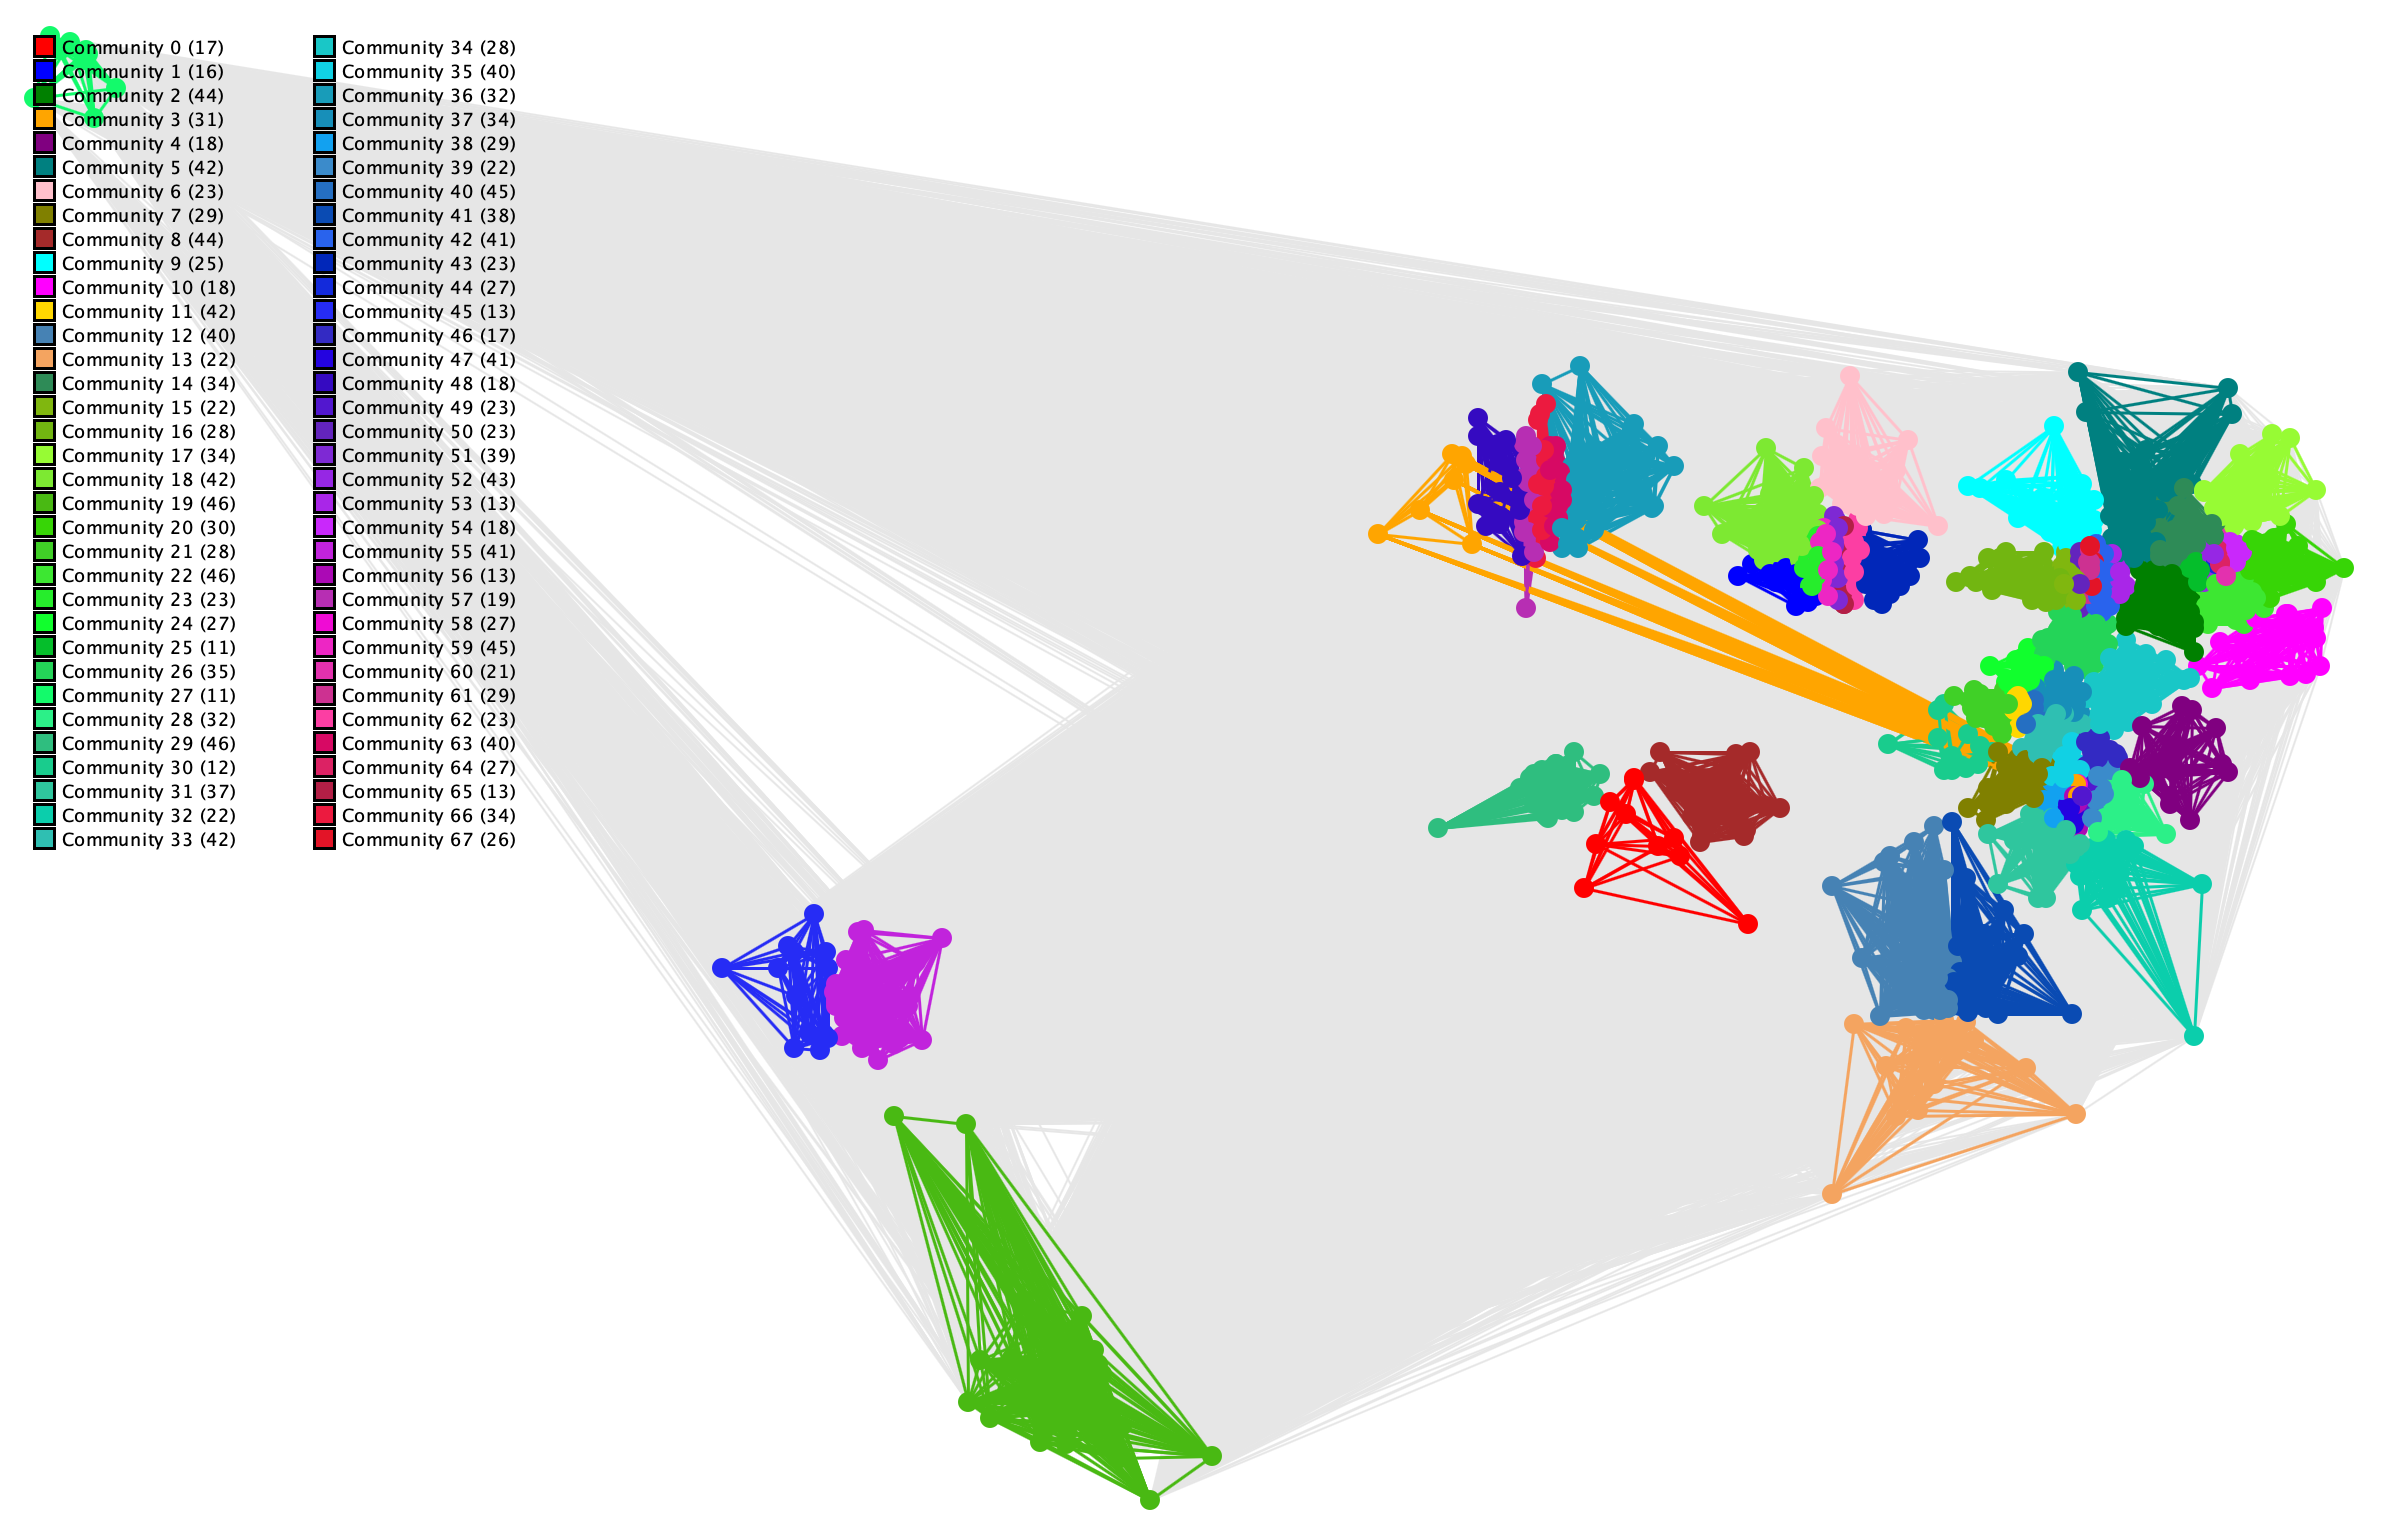
\includegraphics[width=0.8\textwidth]{img/leiden_complete2}
\caption{Leiden algorithm applied to a complete graph representation. The high number of edges between all student locations illustrates the computational expensiveness of the complete graph approach, making it less practical for large-scale transportation planning.}
\label{fig:leiden_complete}
\end{figure}

We primarily utilized the Leiden algorithm (see Section~\ref{subsec:LeidenAlgorithm}), which optimizes modularity to find densely connected communities with its refinement phase ensuring well-connected clusters. The algorithm was configured with adaptive resolution to produce balanced clusters.

\begin{table}[h]
\centering

\label{tab:leiden_complete_example}
\begin{tabular}{|c|c|c|c|c|c|c|c|}
\hline
\textbf{Comm.} & \textbf{Students}  &  \textbf{Distance} & \textbf{Fuel} & \textbf{Fuel Cost} & \textbf{Total} \\
\textbf{ID} & & \textbf{(km)} & \textbf{(L)} & \textbf{(TL)} & \textbf{Cost (TL)} \\
\hline
54 & 18  & 45.70 & 18.74 & 849.35 & 2445.35 \\
\hline
\end{tabular}
\caption{Example of a clustered community using Leiden algorithm on complete graph}
\end{table}

The clusters from the complete graph often required post-processing to merge small communities and split oversized ones, ensuring adherence to the capacity constraints. This post-processing uses geographic proximity to guide the merging and splitting operations, prioritizing the combination of communities that are spatially close while ensuring each resulting community remains within the capacity limits.

\subsubsection{Minibus Solution for Imbalanced Clusters}
\label{subsubsec:minibus_solution}

When analyzing the complete graph representation, we observed that the resulting clusters were often imbalanced, with many clusters having fewer than 25 students. This created an inefficiency in the transportation system, as standard buses with a capacity of 50 students would be underutilized. To address this issue, we implemented a vehicle type allocation strategy that assigns minibuses (with a maximum capacity of 25 students) to smaller clusters containing 10-25 students, while standard buses were allocated to larger clusters with 26-50 students. This differentiated approach resulted in significant cost savings due to the lower fuel consumption of minibuses compared to standard buses. However, it's important to note that IZTECH currently does not have minibuses in its fleet, only standard buses. This limitation motivates our exploration of alternative graph construction methods that might produce more balanced clusters suitable for the existing bus fleet.

\subsection{Clustering Sparse Graph Representation}
\label{subsec:clustering_sparse}

The sparse graph representations required specialized clustering approaches to effectively partition the transportation network. In our implementation, each node in the graph represents a specific student's residential address in Izmir, with geographical coordinates (latitude and longitude) obtained from our synthetic dataset. The edges represent potential transportation links between student locations, with weights based on the Euclidean distance between points.

For our transportation network analysis, we implemented three clustering algorithms with specific configurations tailored to the IZTECH student transportation problem. All implementations included specialized vehicle allocation logic that assigns buses with our capacity constraints (10-50 students per bus), optimizing for both fleet size and route efficiency.

\subsubsection{Performing Spectral Clustering on Sparse Graph Representations of IZTECH}
\label{subsubsec:spectral_implementation}

For the Spectral clustering implementation, we focused on optimizing the eigendecomposition process for large sparse matrices. Our implementation used the normalized Laplacian matrix and employed an adaptive approach to determine the number of clusters. We developed a custom post-processing step that enforces our specific bus capacity constraints (10-50 students) by iteratively merging small clusters or splitting oversized ones based on geographic proximity.

\begin{figure}[htbp]
\centering
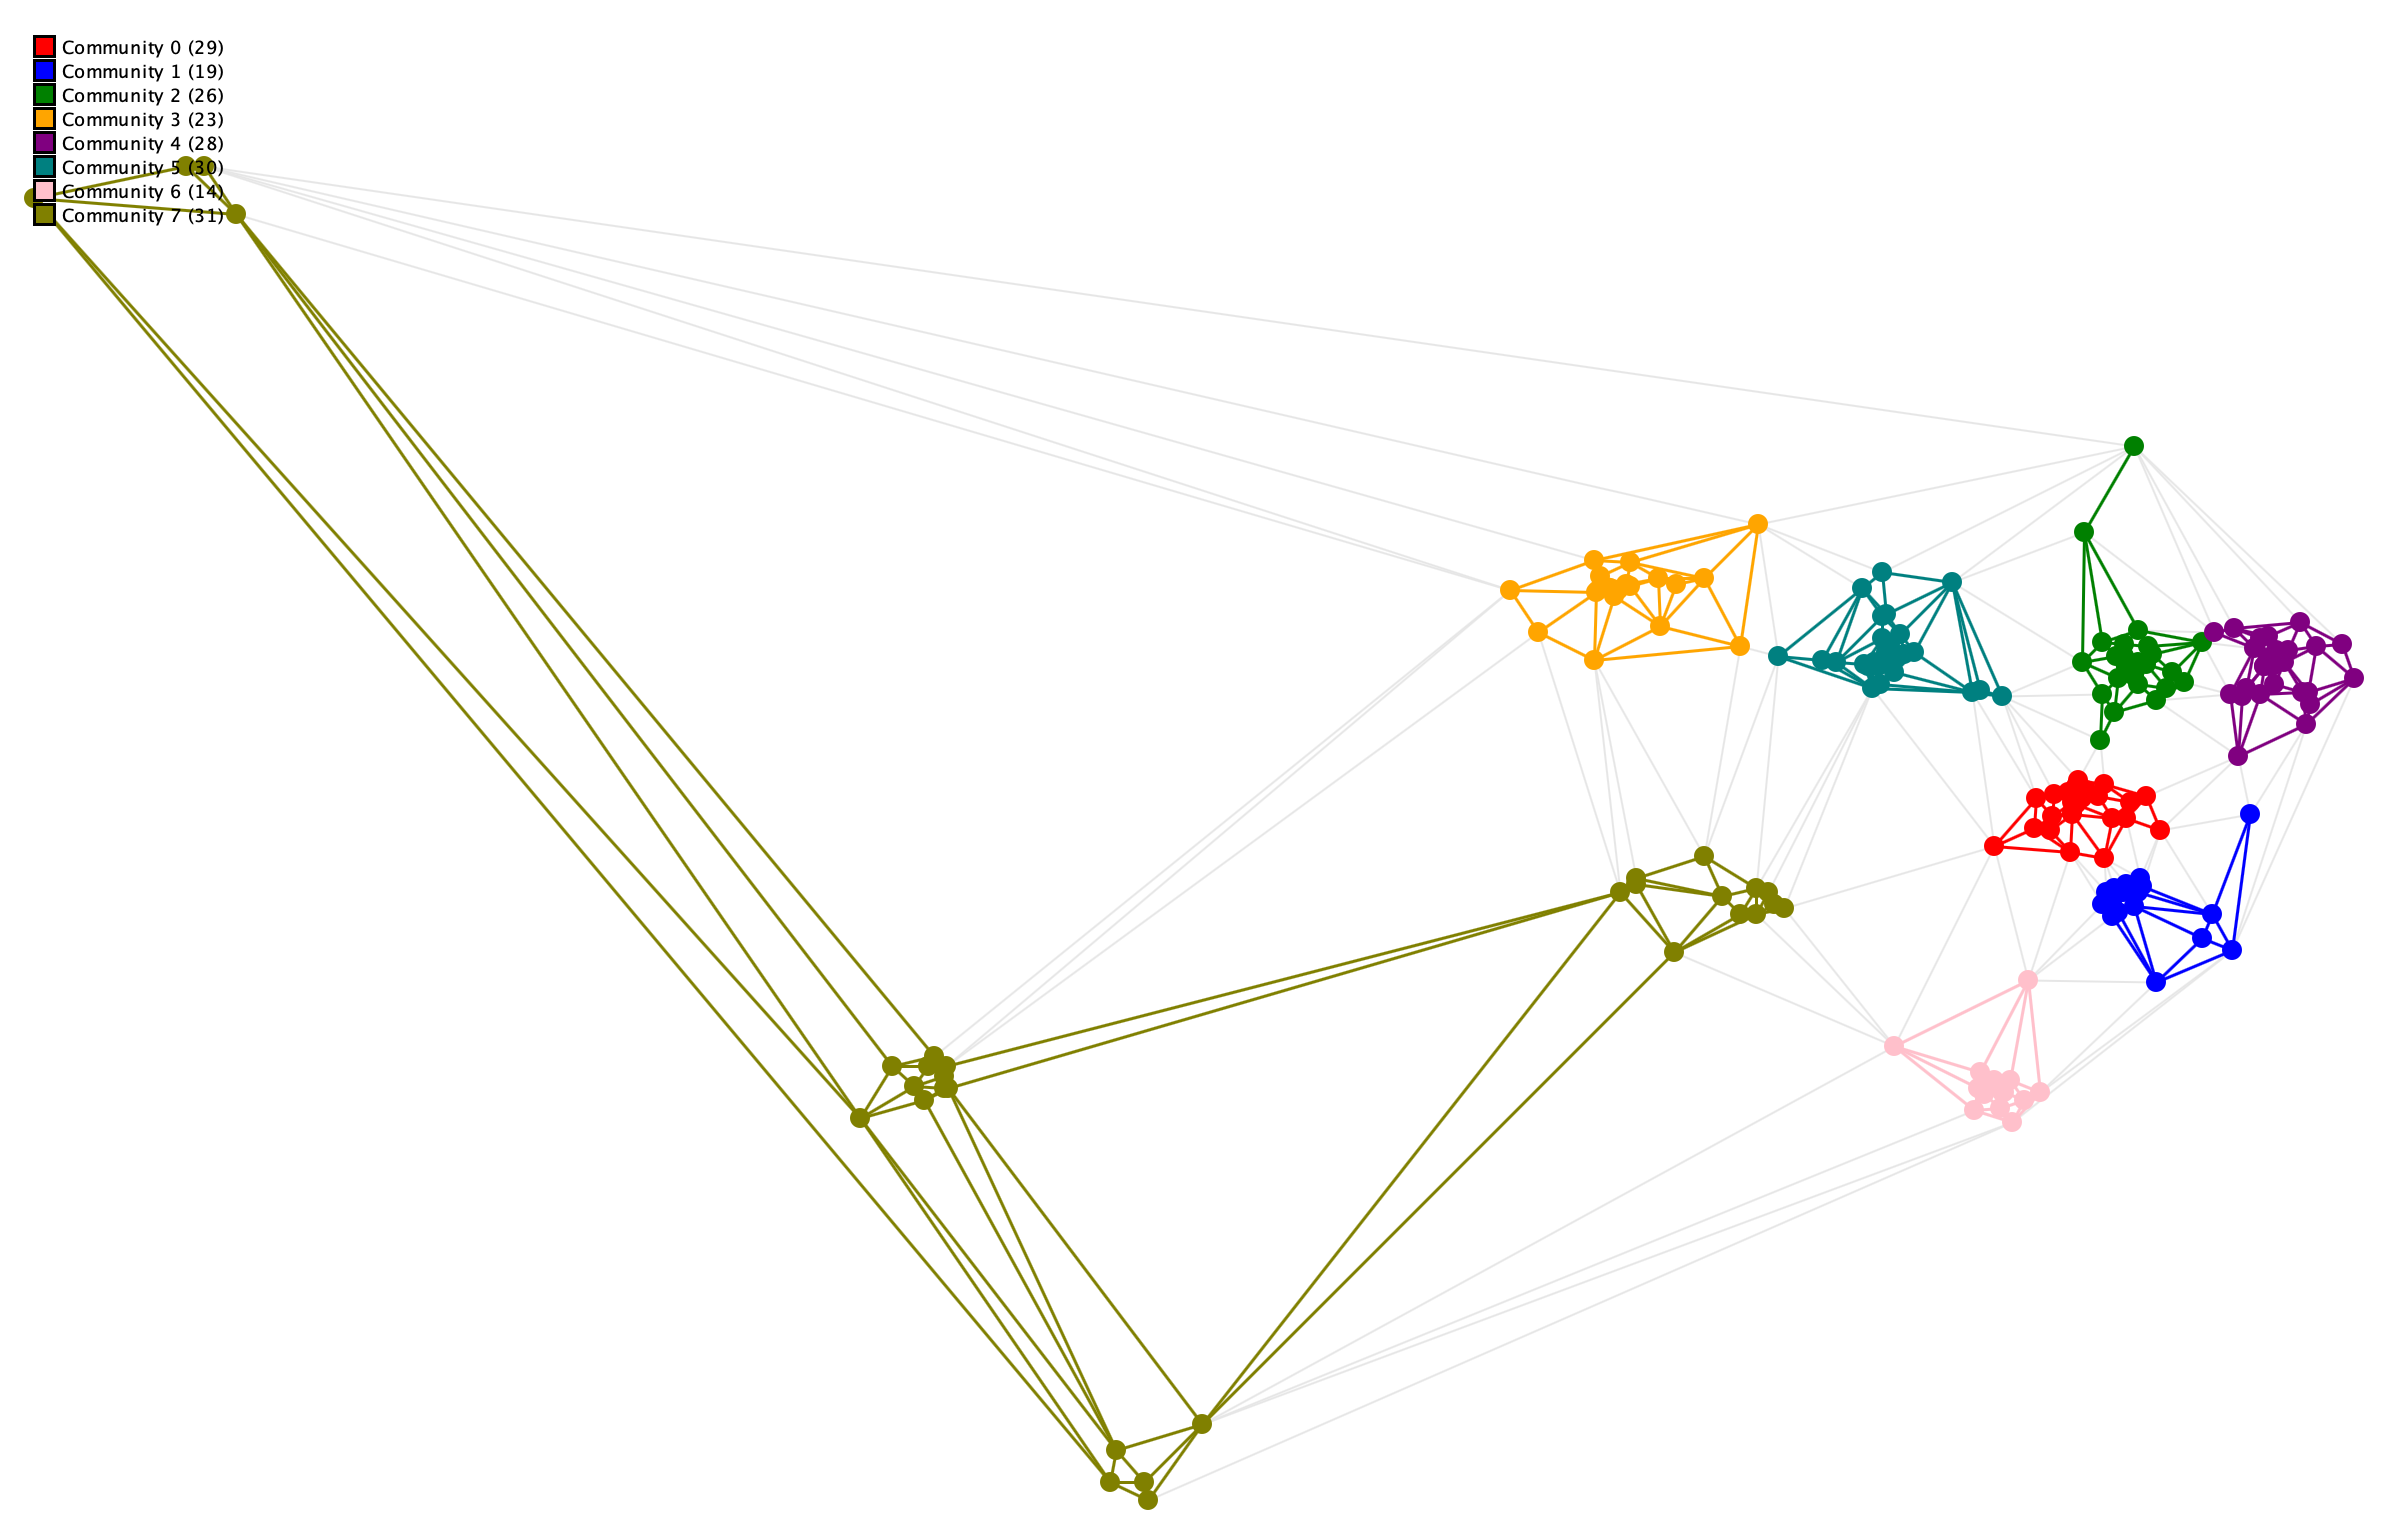
\includegraphics[width=0.5\textwidth]{./img/Spectral_Delaunay}
\vspace{0.5cm}

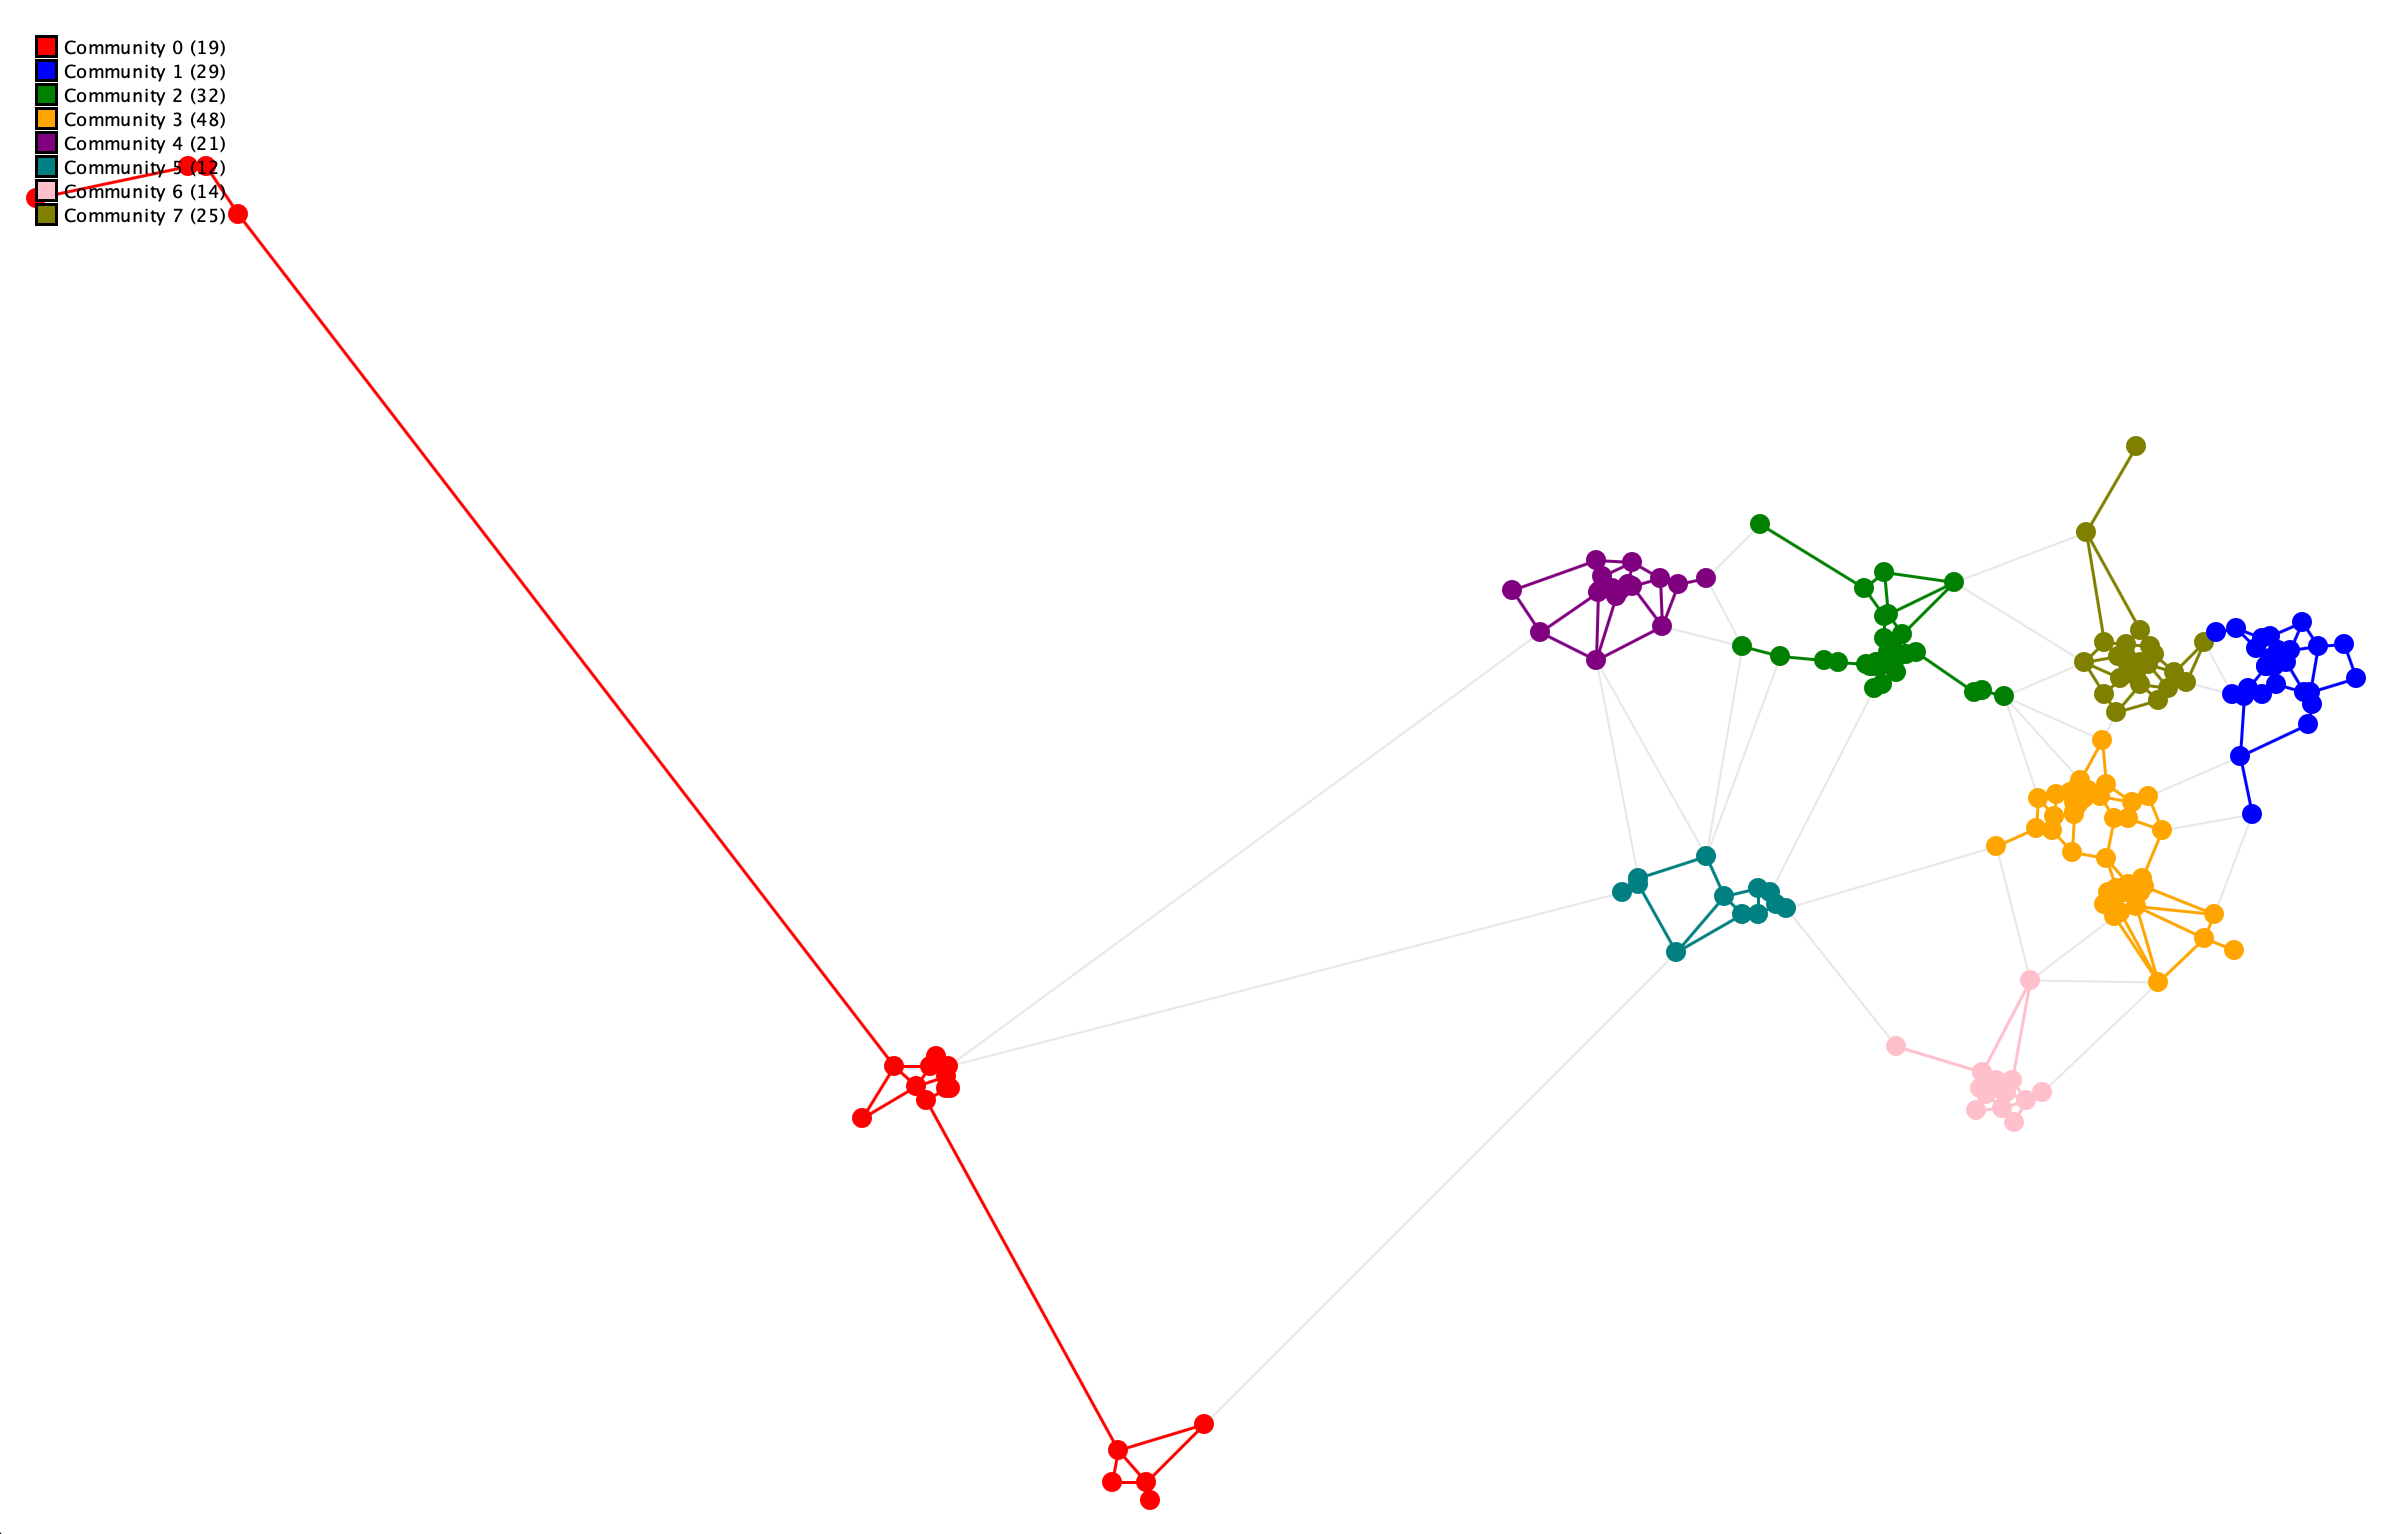
\includegraphics[width=0.5\textwidth]{./img/Spectral_Gabriel}
\vspace{0.5cm}

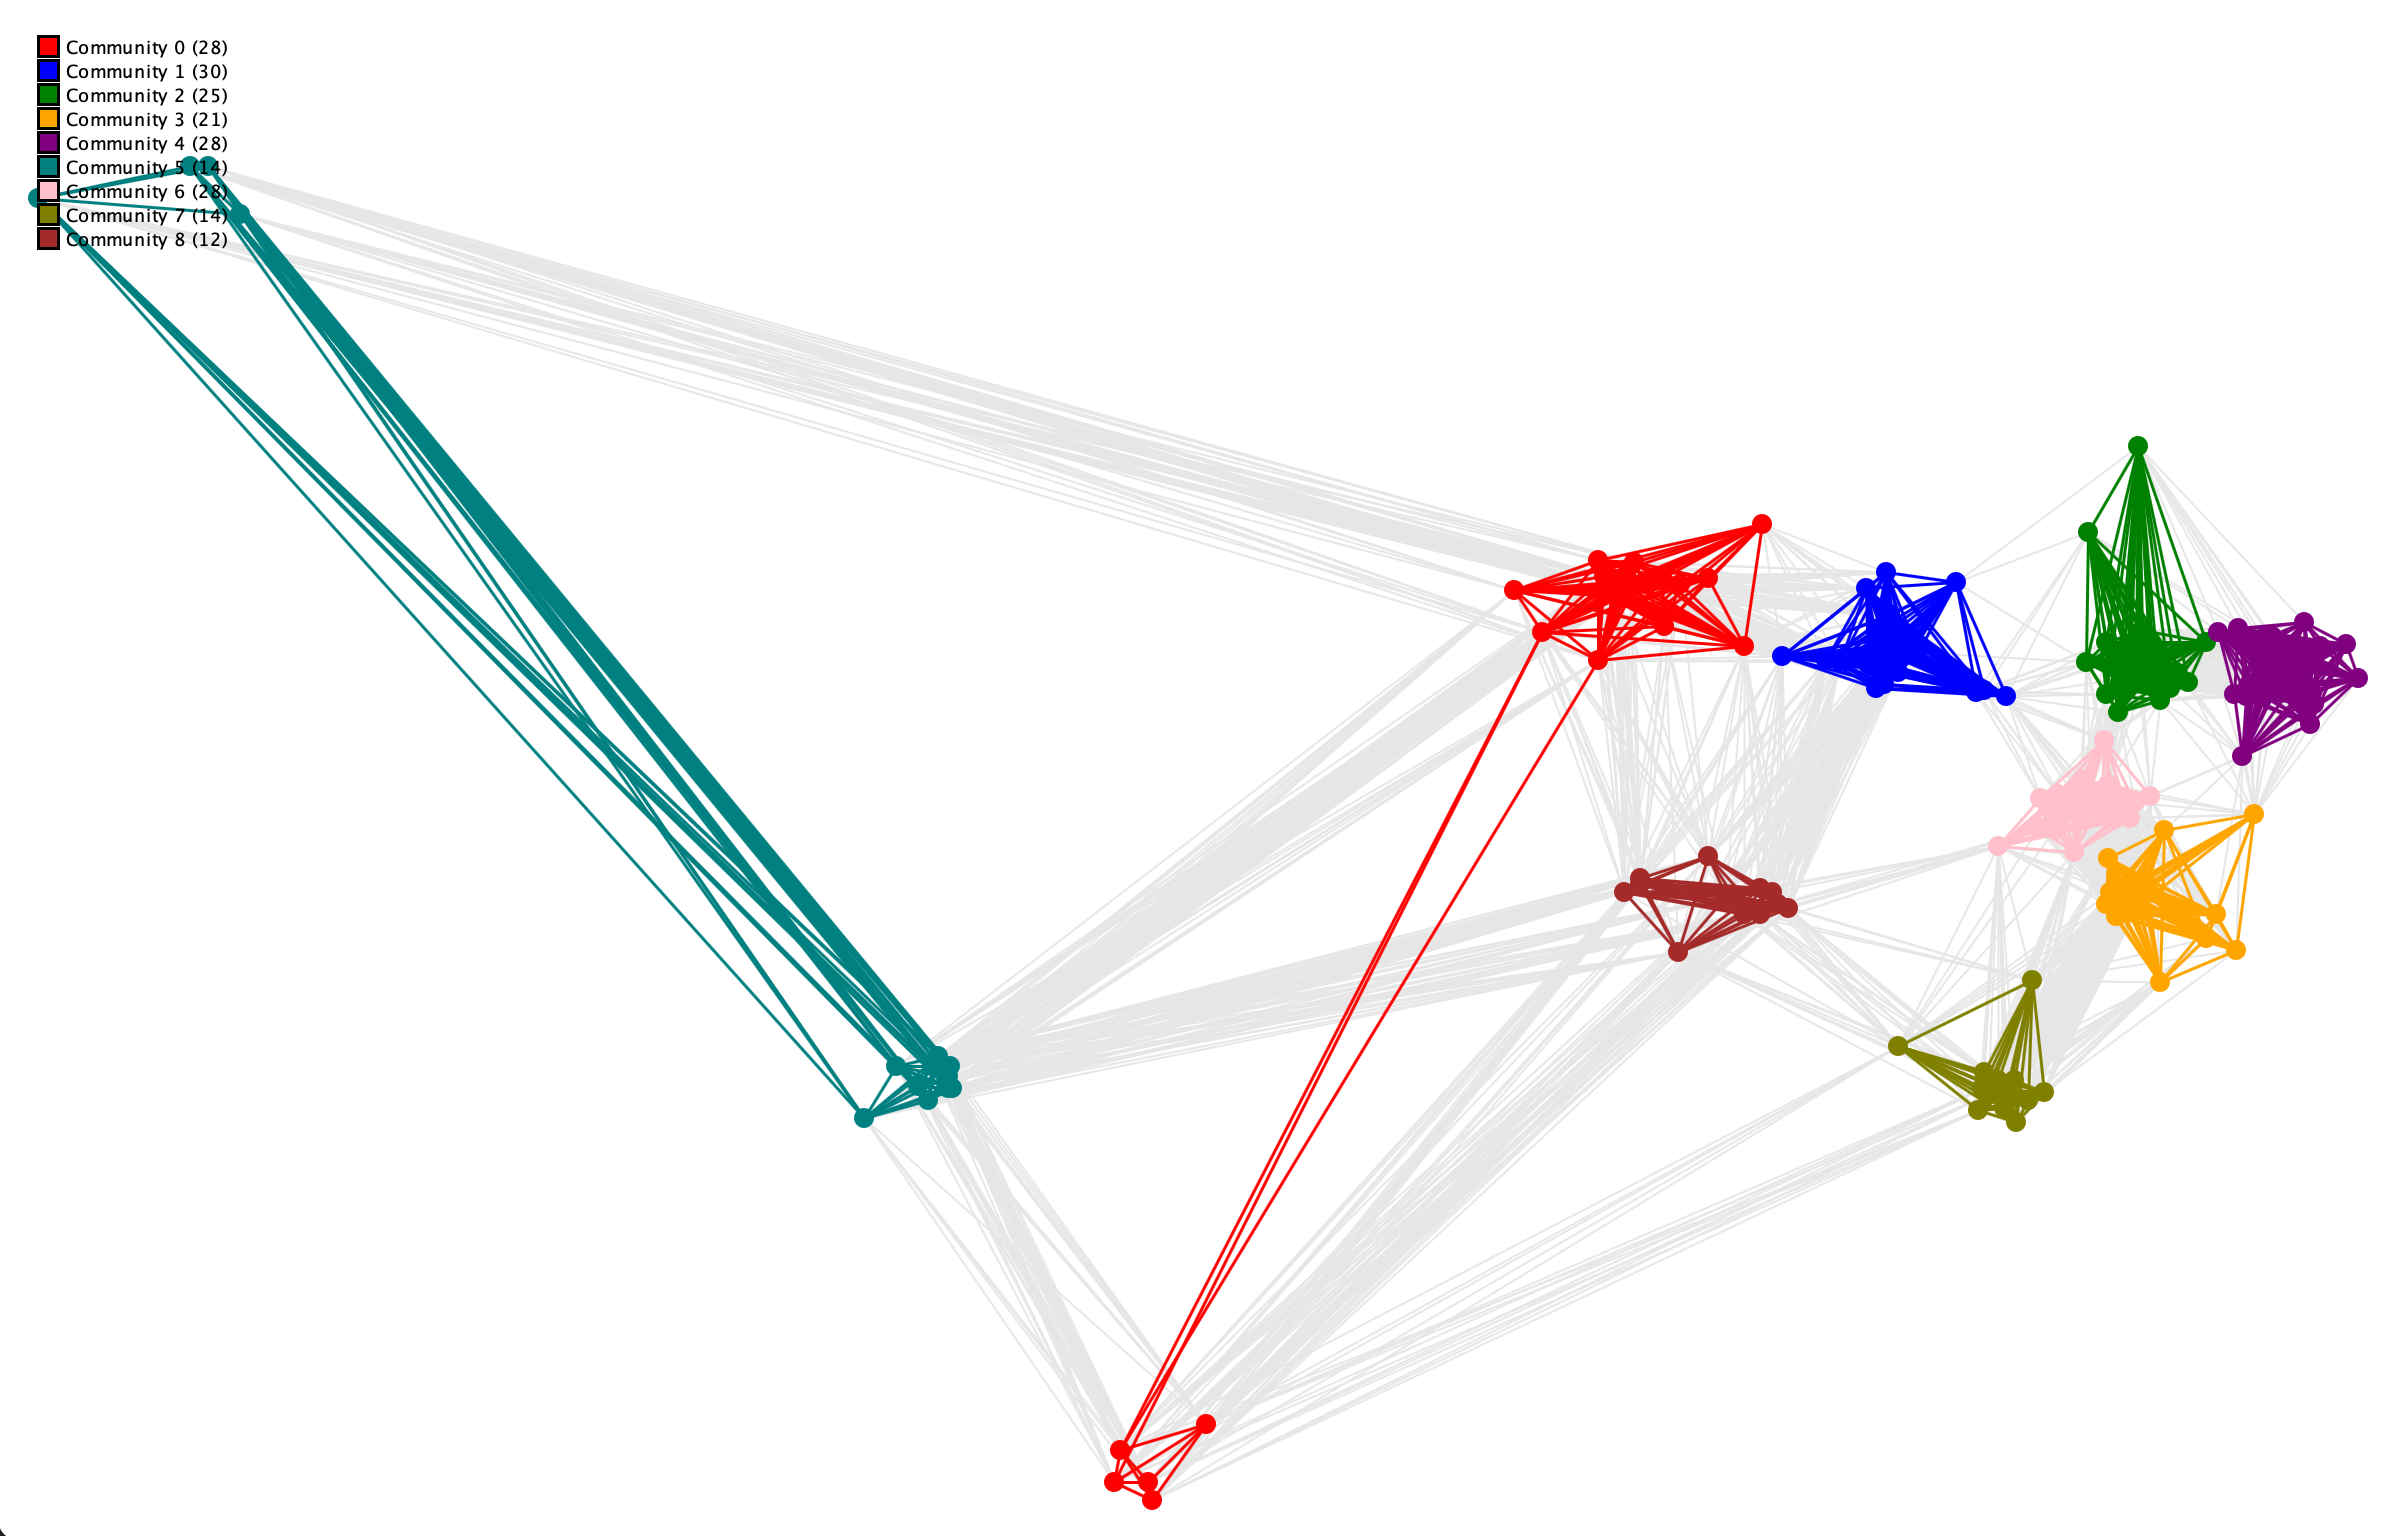
\includegraphics[width=0.5\textwidth]{./img/Spectral_K}

\caption{Spectral clustering applied to different sparse graph representations (top: Delaunay, middle: Gabriel, bottom: K-Nearest) with 200 student locations.}
\label{fig:spectral_clustering}
\end{figure}

Figure \ref{fig:spectral_clustering} illustrates the application of Spectral clustering to three different sparse graph representations. Each point represents a student address, and colors indicate cluster assignments. With Delaunay triangulation, clusters form well-connected regions with smoother boundaries; with Gabriel graph, clusters are more compact but show increased fragmentation; with K-Nearest Neighbors (k=30), clusters demonstrate better local coherence but with some outlier assignments.

As shown in these visualizations, our Spectral clustering implementation tends to create clusters with clear geographical boundaries. This demonstrates how the algorithm's eigenvalue-based dimensionality reduction effectively captures the global structure of Izmir's transportation network. The clusters formed by spectral clustering typically have larger student counts, which aligns with the algorithm's natural tendency to identify major structural divisions in the graph before finer details.

The spectral approach is particularly suitable for transportation planning scenarios that prioritize minimizing the number of vehicles while accepting potentially longer routes per vehicle.

\subsubsection{Performing Leiden Clustering on Sparse Graph Representations of IZTECH}
\label{subsubsec:leiden_implementation}

For the Leiden algorithm implementation, we modified the original algorithm to better handle transportation constraints. Specifically, we incorporated a custom quality function that considers both community modularity and geographic compactness. We adjusted the resolution parameter based on the sparsity of the underlying graph, with values ranging from 0.8 for complete graphs to 1.2 for sparser representations. This adaptation allowed the algorithm to find well-connected communities while respecting the spatial constraints inherent in transportation planning.

\begin{figure}[H]
\centering
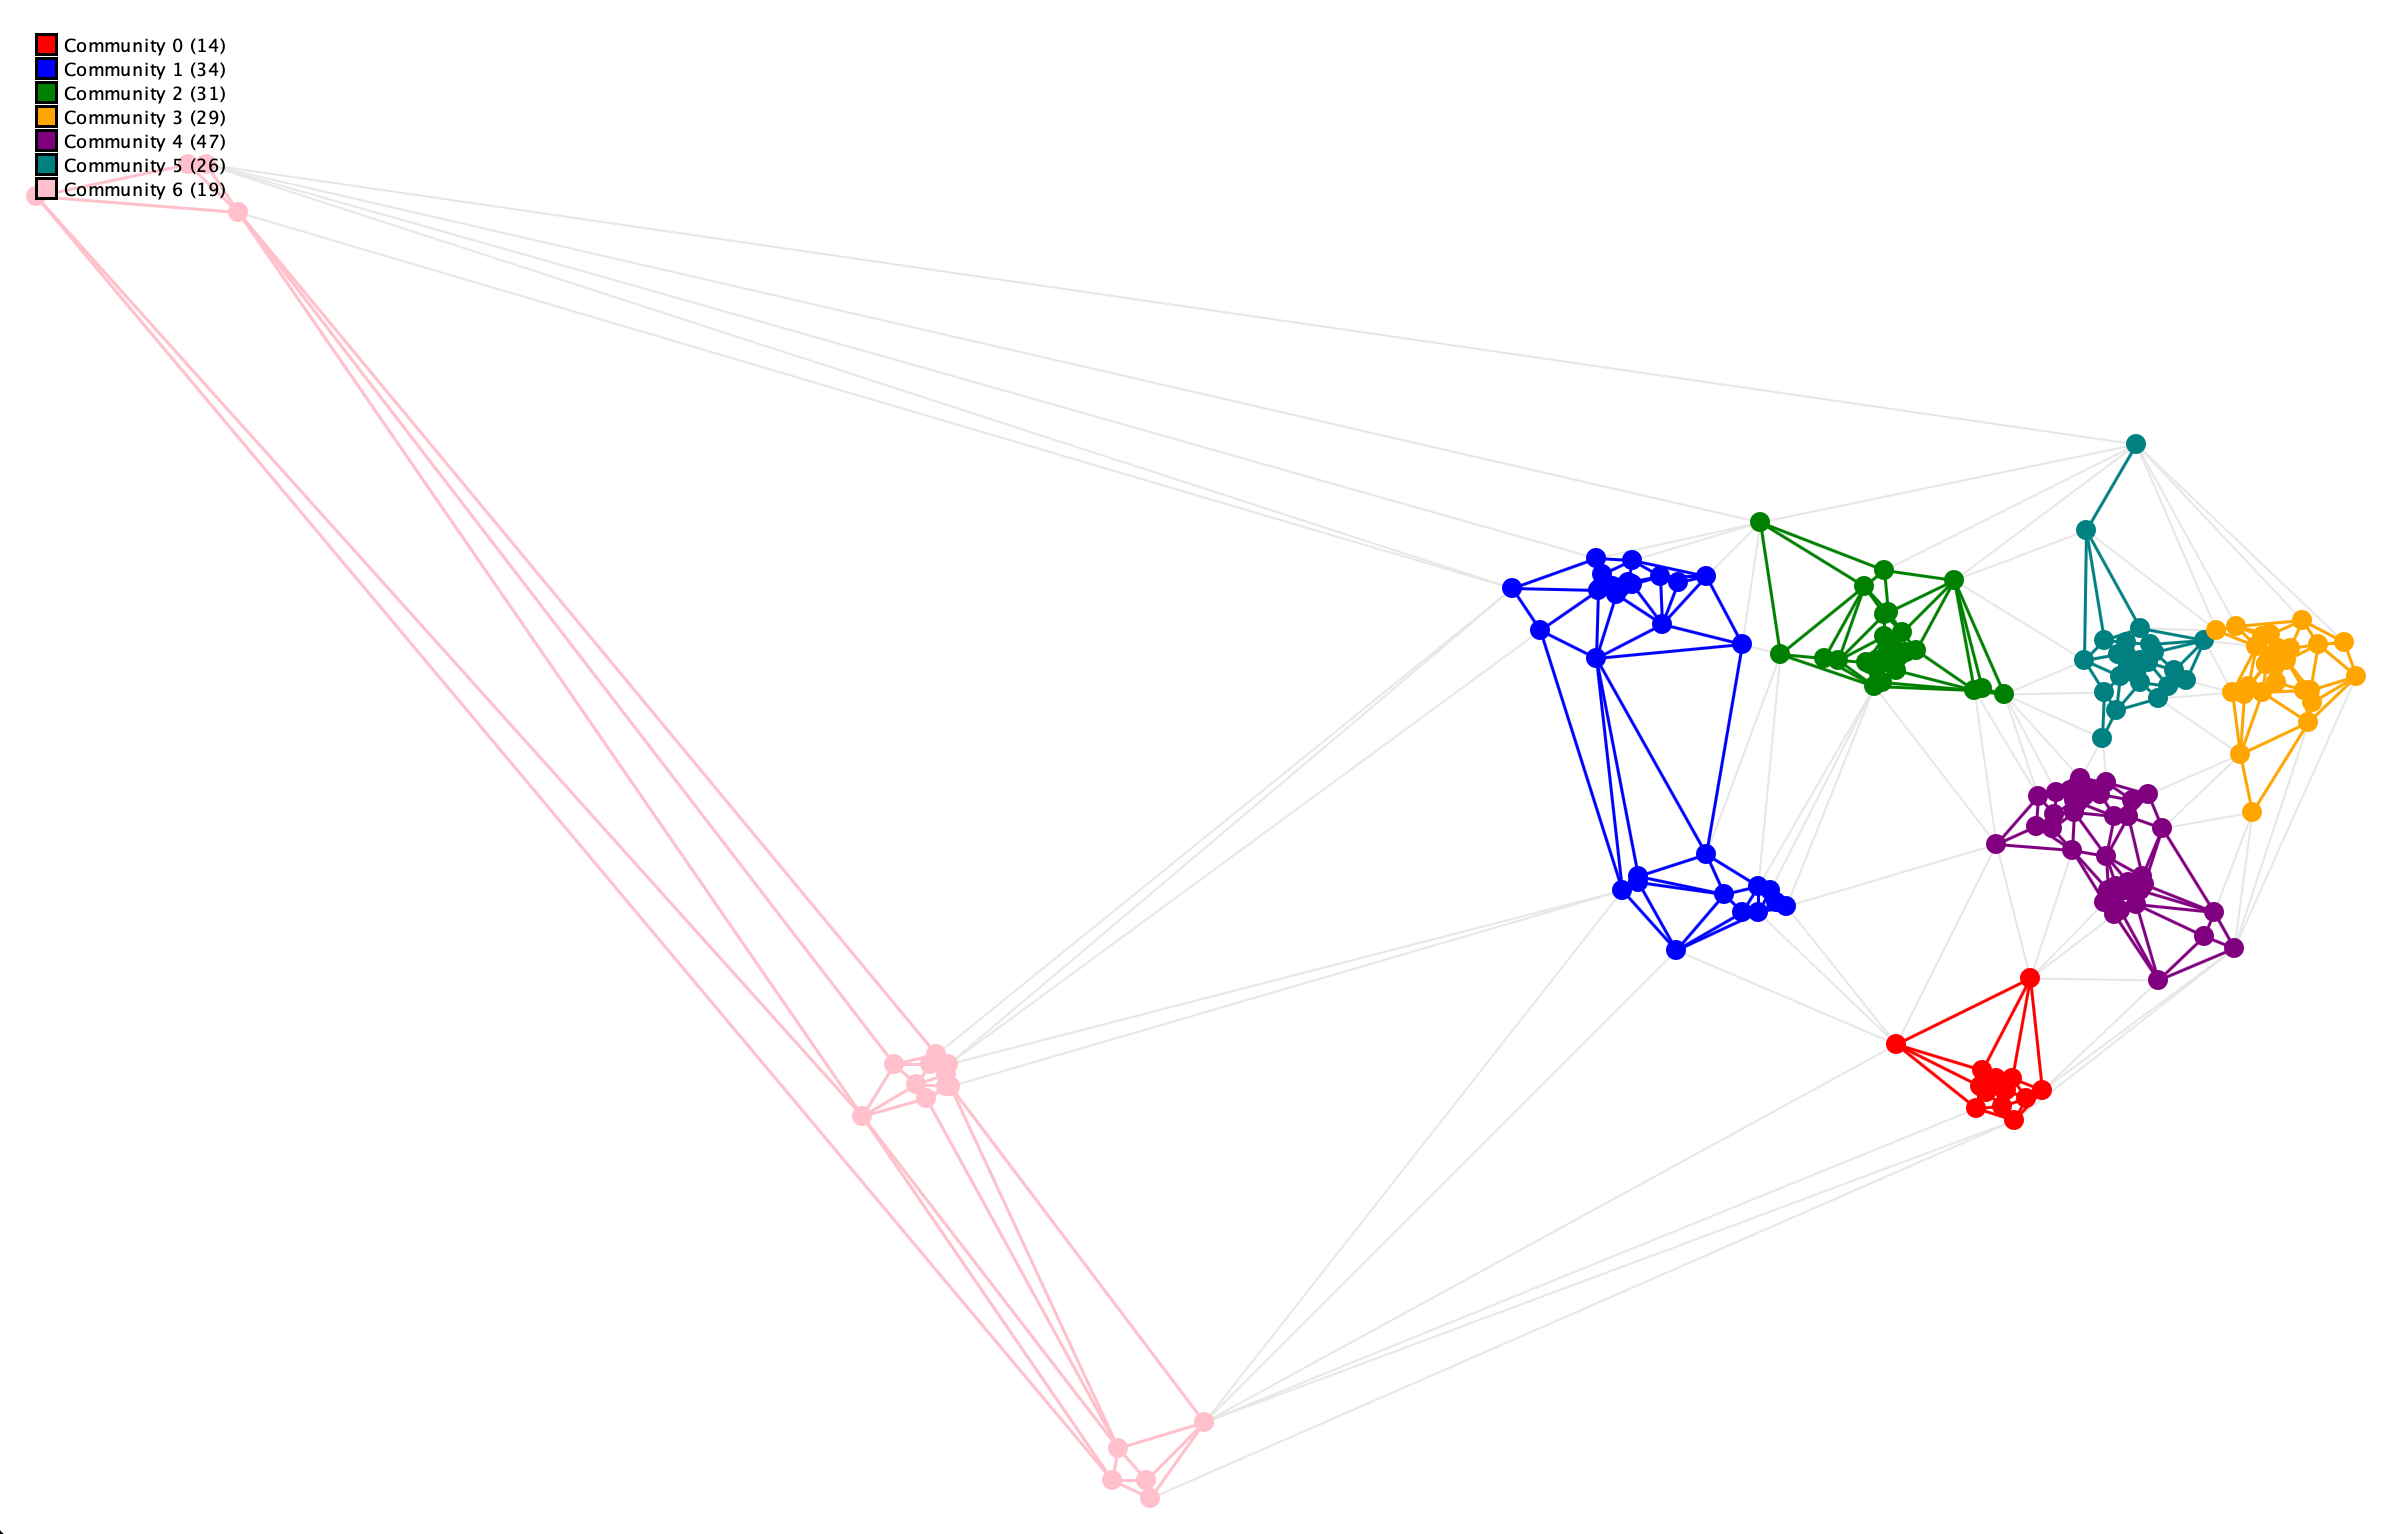
\includegraphics[width=0.5\textwidth]{./img/Leiden_Delaunay}
\vspace{0.5cm}

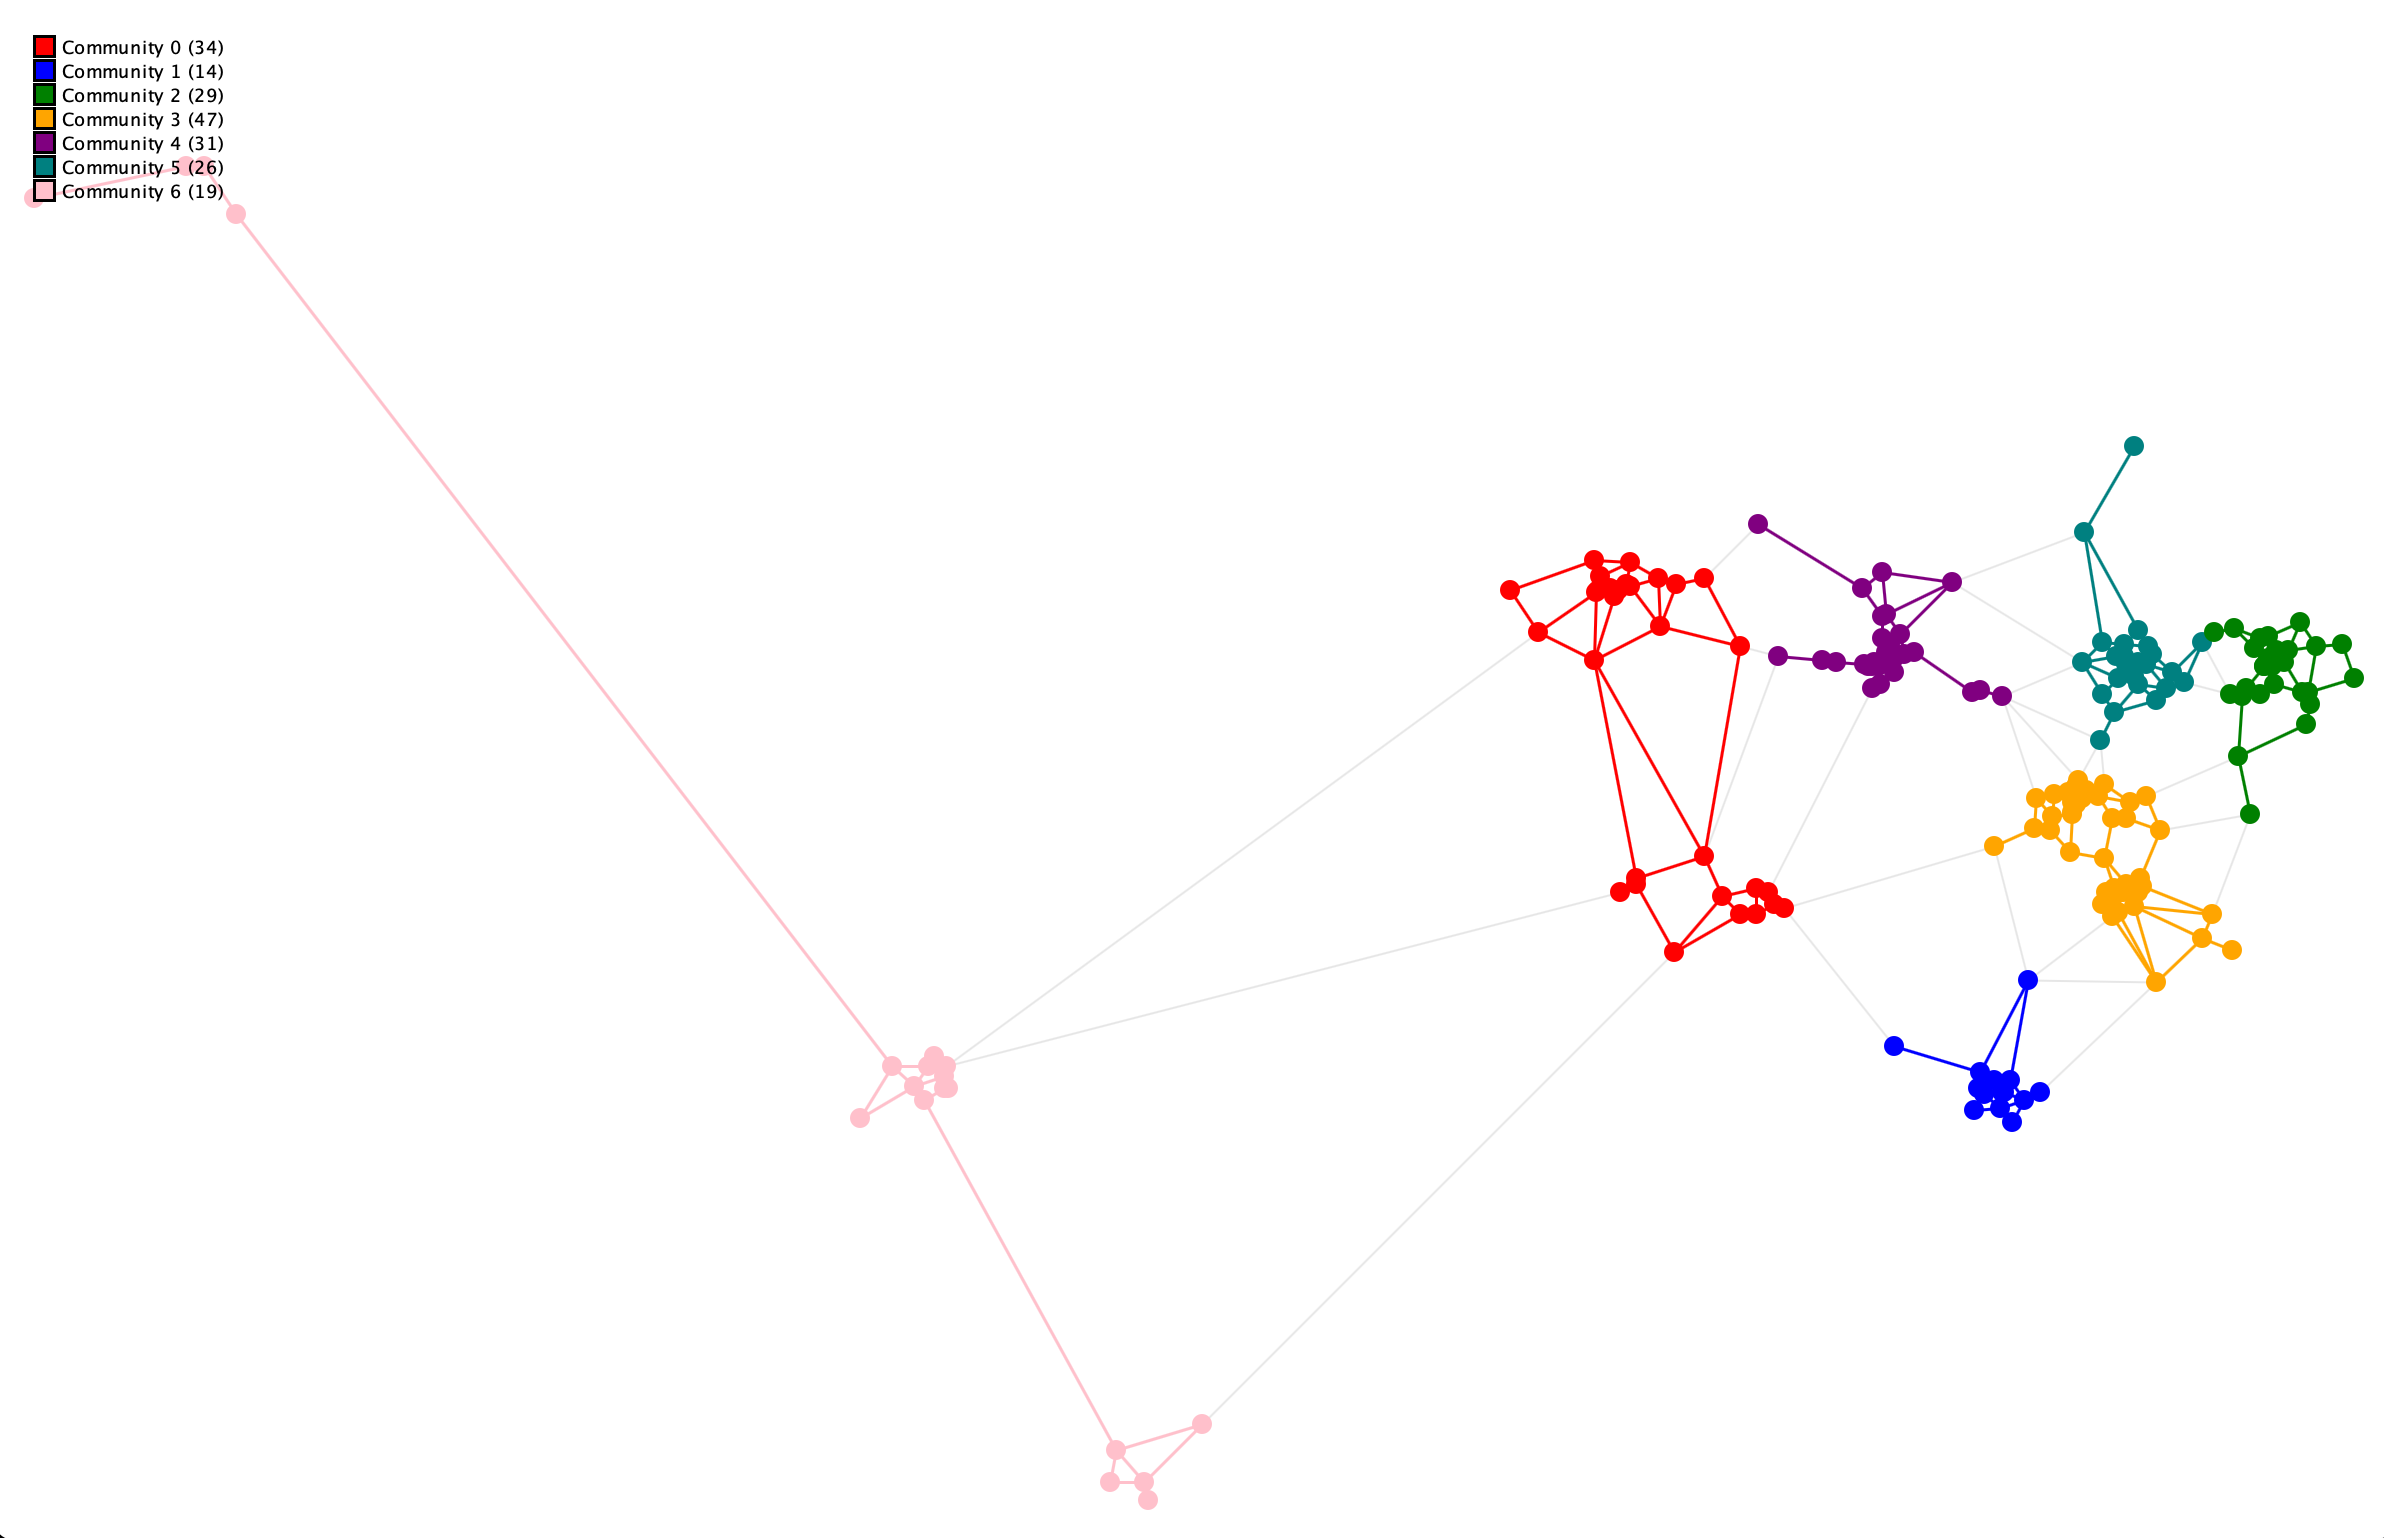
\includegraphics[width=0.5\textwidth]{./img/Leiden_Gabriel}
\vspace{0.5cm}

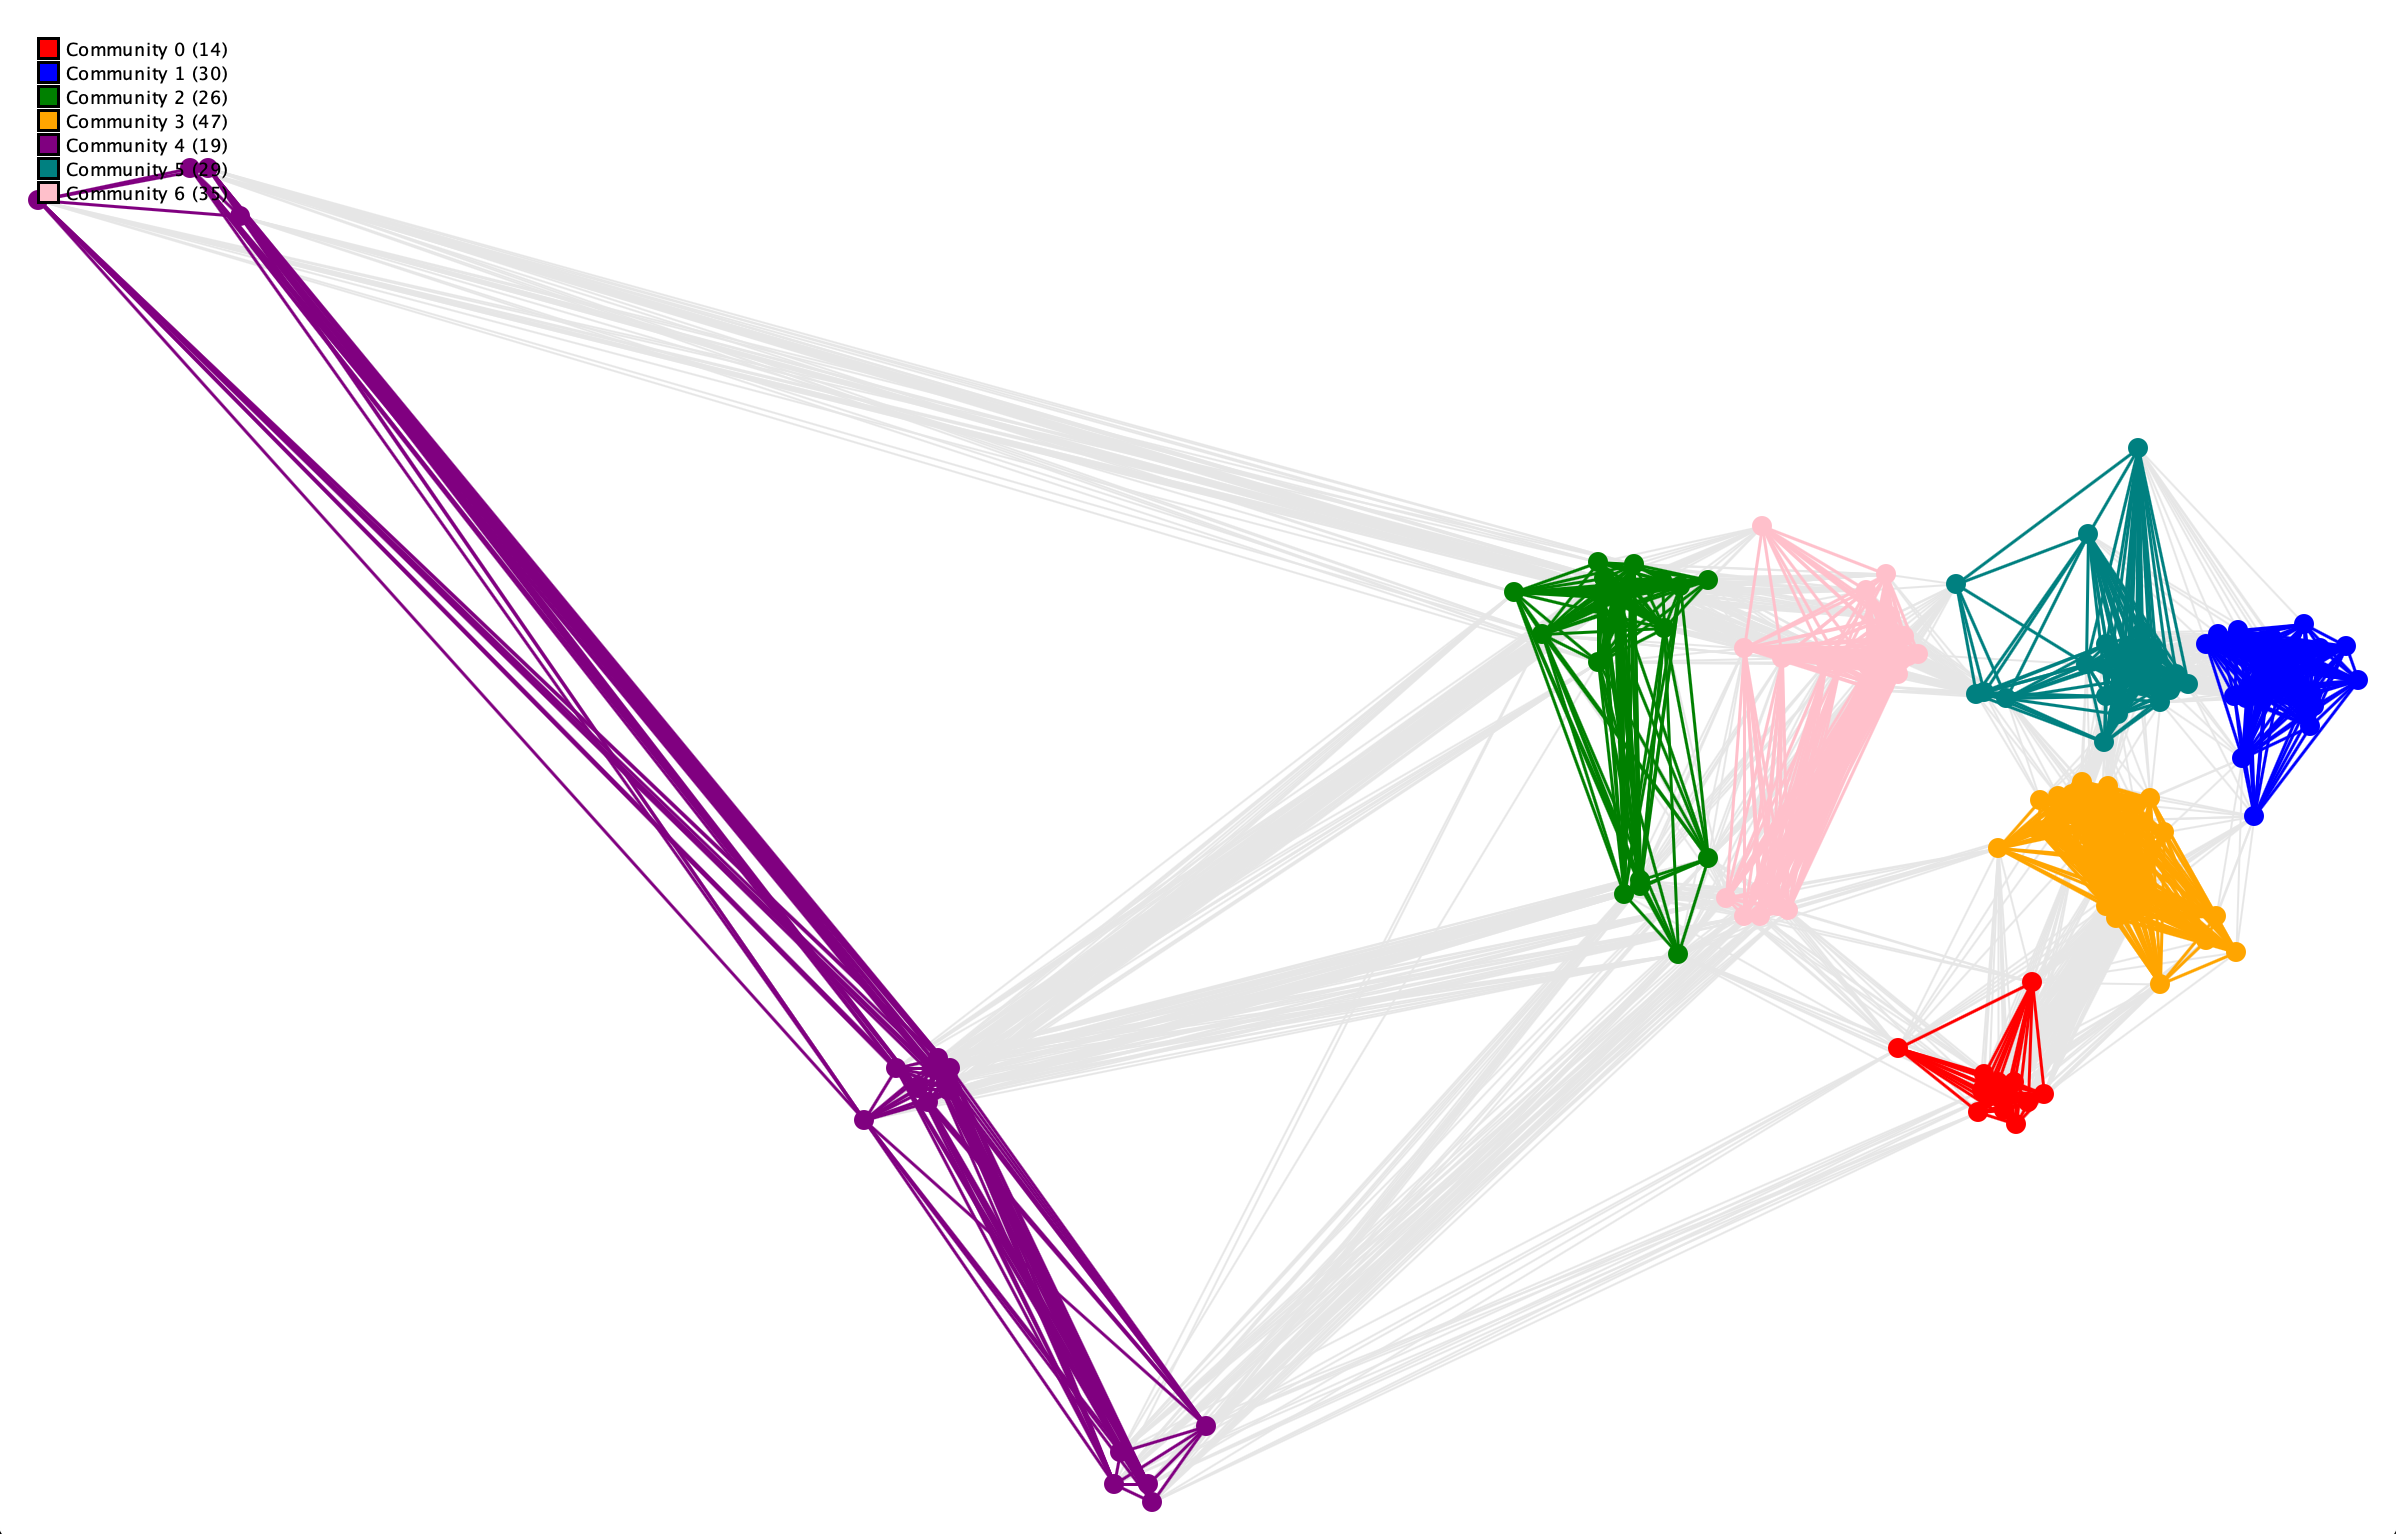
\includegraphics[width=0.5\textwidth]{./img/Leiden_K}

\caption{Leiden algorithm applied to different sparse graph representations (top: Delaunay, middle: Gabriel, bottom: K-Nearest) with 200 student locations.}
\label{fig:leiden_clustering}
\end{figure}

Figure \ref{fig:leiden_clustering} shows the clustering results of our Leiden algorithm implementation across three graph types. On Delaunay triangulation, Leiden identifies geographically coherent communities with balanced sizes; on Gabriel graph, the algorithm forms more compact clusters with clear boundaries; on K-Nearest Neighbors (k=30), Leiden captures local density variations, creating more clusters in densely populated areas and larger clusters in sparse regions.

The Leiden algorithm demonstrates effectiveness at identifying meaningful communities in the transportation network. The visualization reveals how our implementation produces clusters that strongly reflect the underlying graph topology while respecting geographical constraints. The smaller, more numerous clusters reflect the algorithm's emphasis on local connectivity and modularity optimization.

A distinctive characteristic of the Leiden implementation is its consistent performance across different sparse graph representations. This consistency stems from the algorithm's refinement phase, which ensures well-connected communities regardless of the initial graph structure. When examining the clusters formed on the Delaunay graph versus those on the Gabriel graph, we observe similar community sizes despite the different edge structures, demonstrating the algorithm's robustness.

The Leiden approach offers a balanced clustering solution for transportation planning, accommodating mixed vehicle fleets while maintaining reasonable geographic coherence within each cluster.

\subsubsection{Performing MVAGC on Sparse Graph Representations of IZTECH}
\label{subsubsec:mvagc_implementation}

Our MVAGC implementation was specifically adapted for geospatial data clustering. Rather than using random sampling for anchor points, we employed a geographically stratified selection process to ensure anchor points were well-distributed across Izmir's districts. This modification improved the algorithm's ability to create geographically coherent clusters. We configured the implementation with approximately 500 anchor points and employed higher-order filtering with a standardized cutoff threshold of 0.25 for ensuring smooth community boundaries.

\begin{figure}[!ht]
\centering
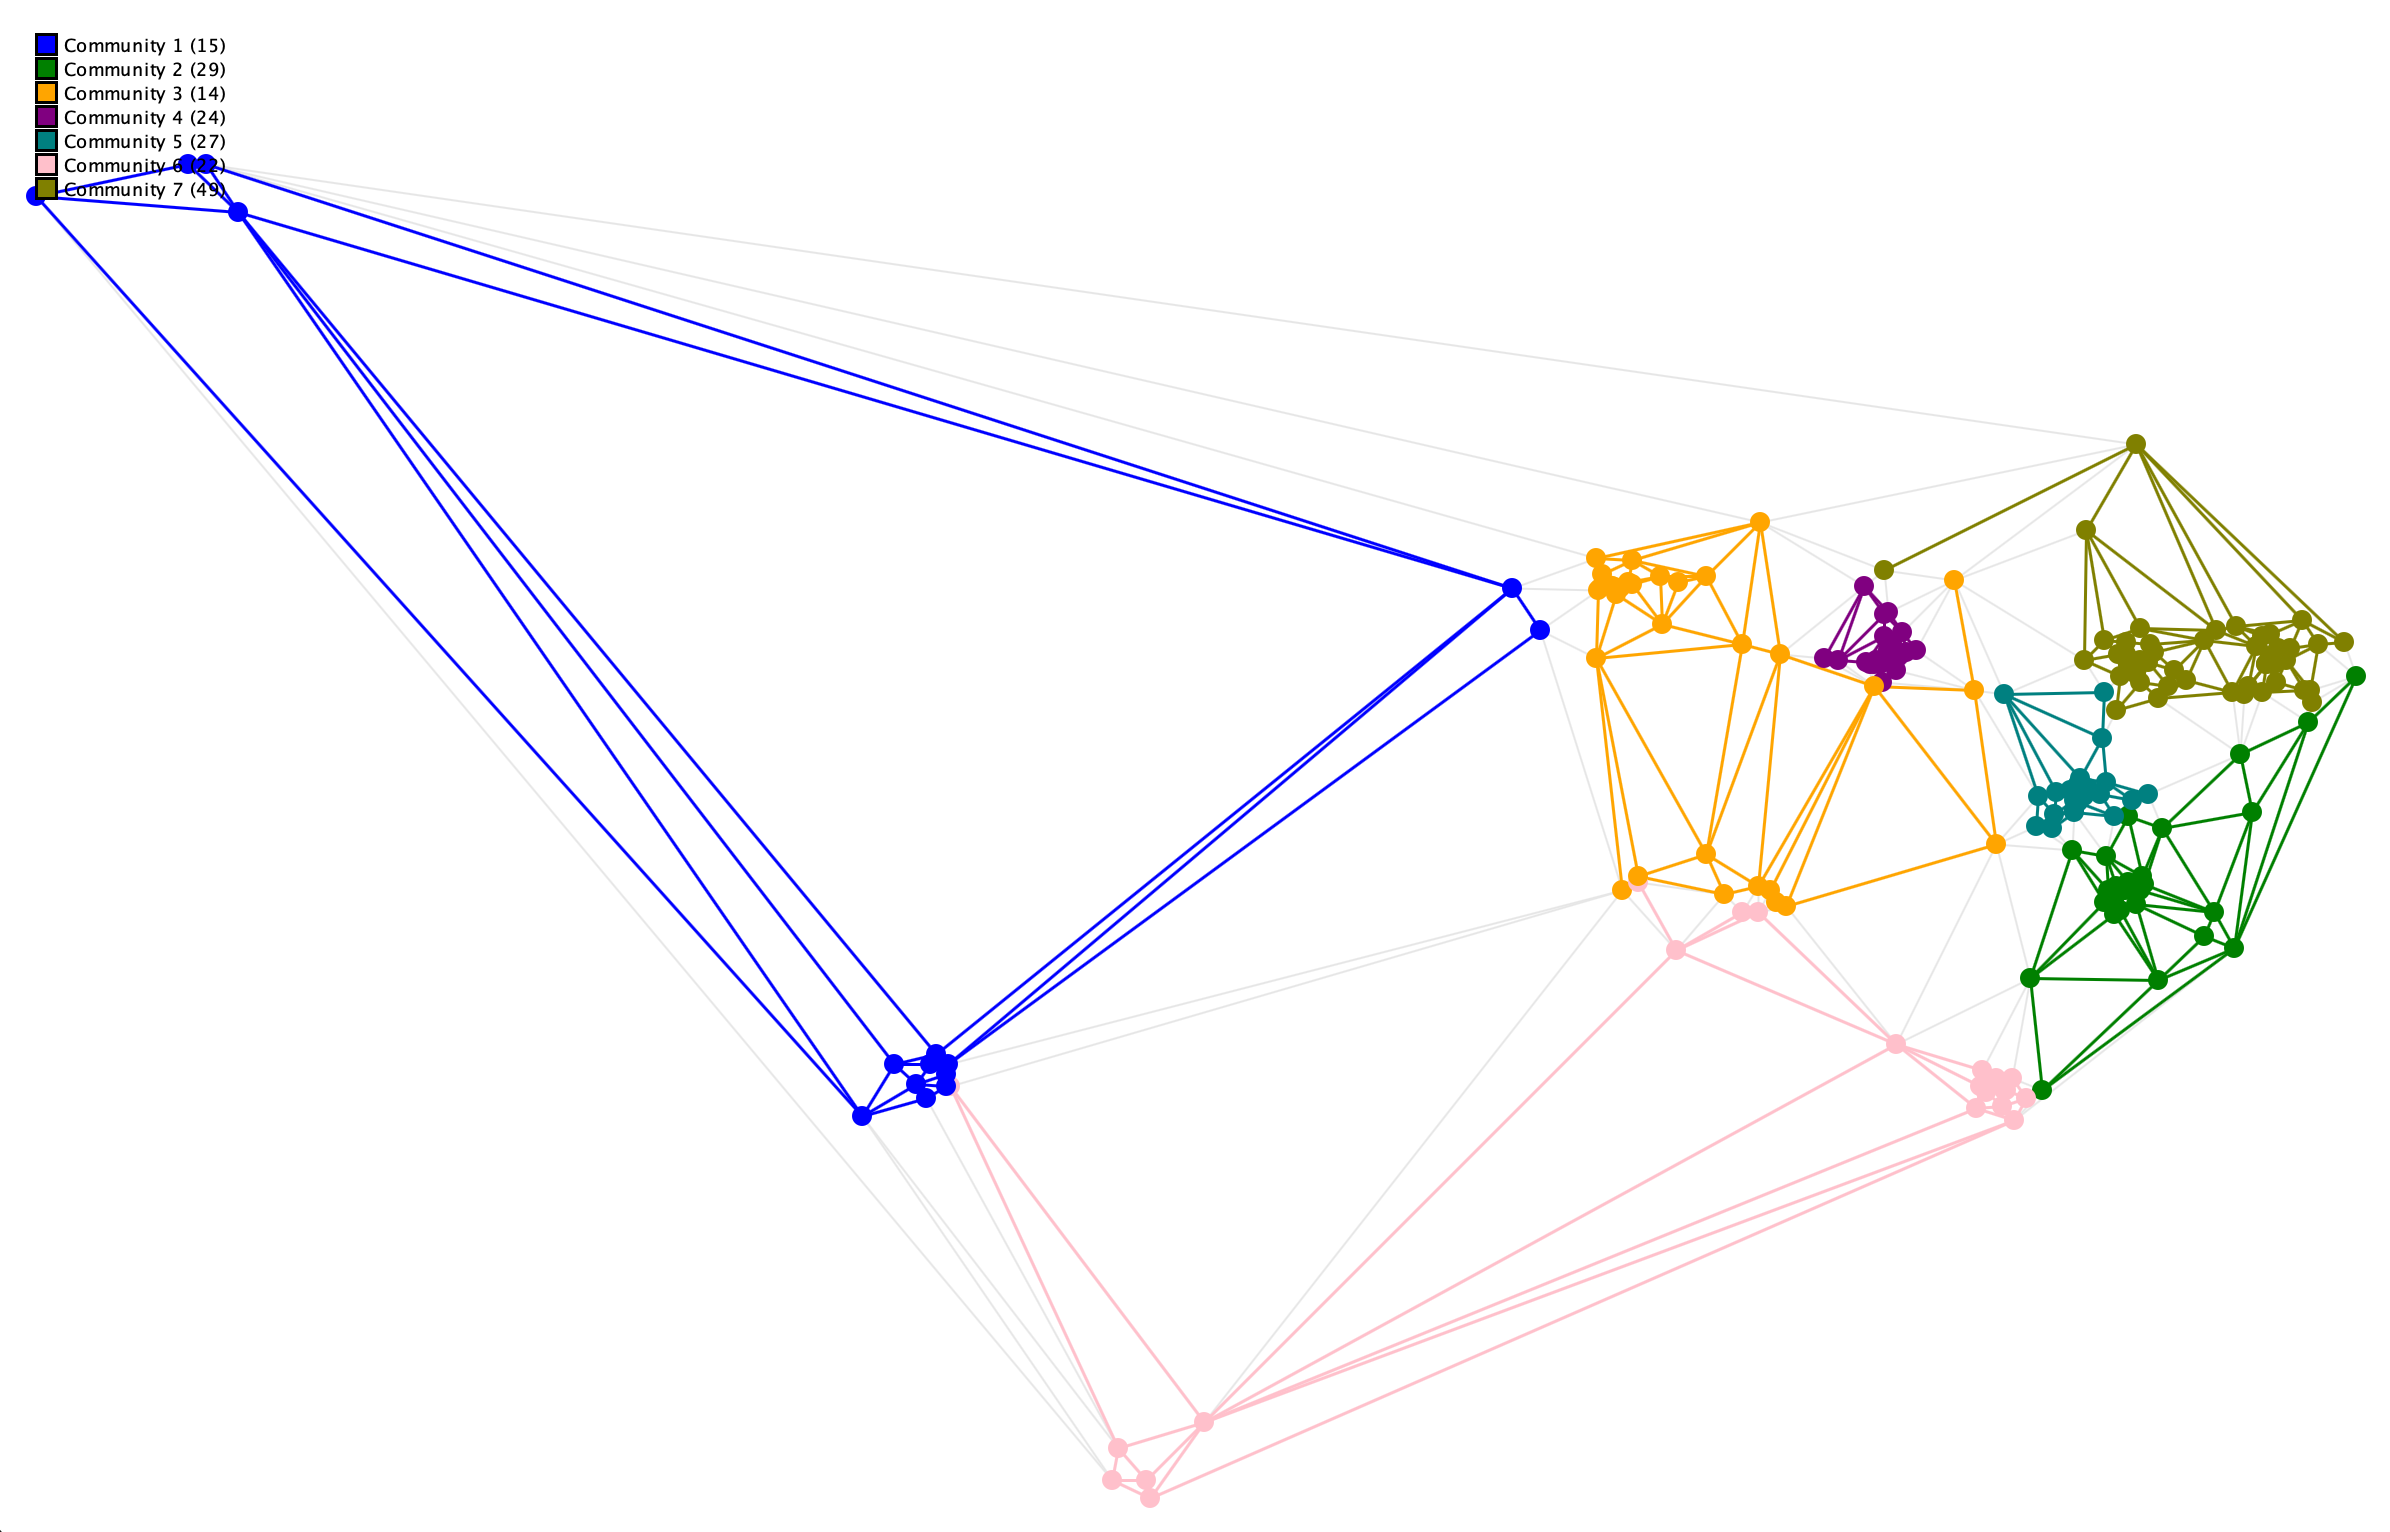
\includegraphics[width=0.5\textwidth]{./img/MVAGC_Delaunay}
\vspace{0.5cm}

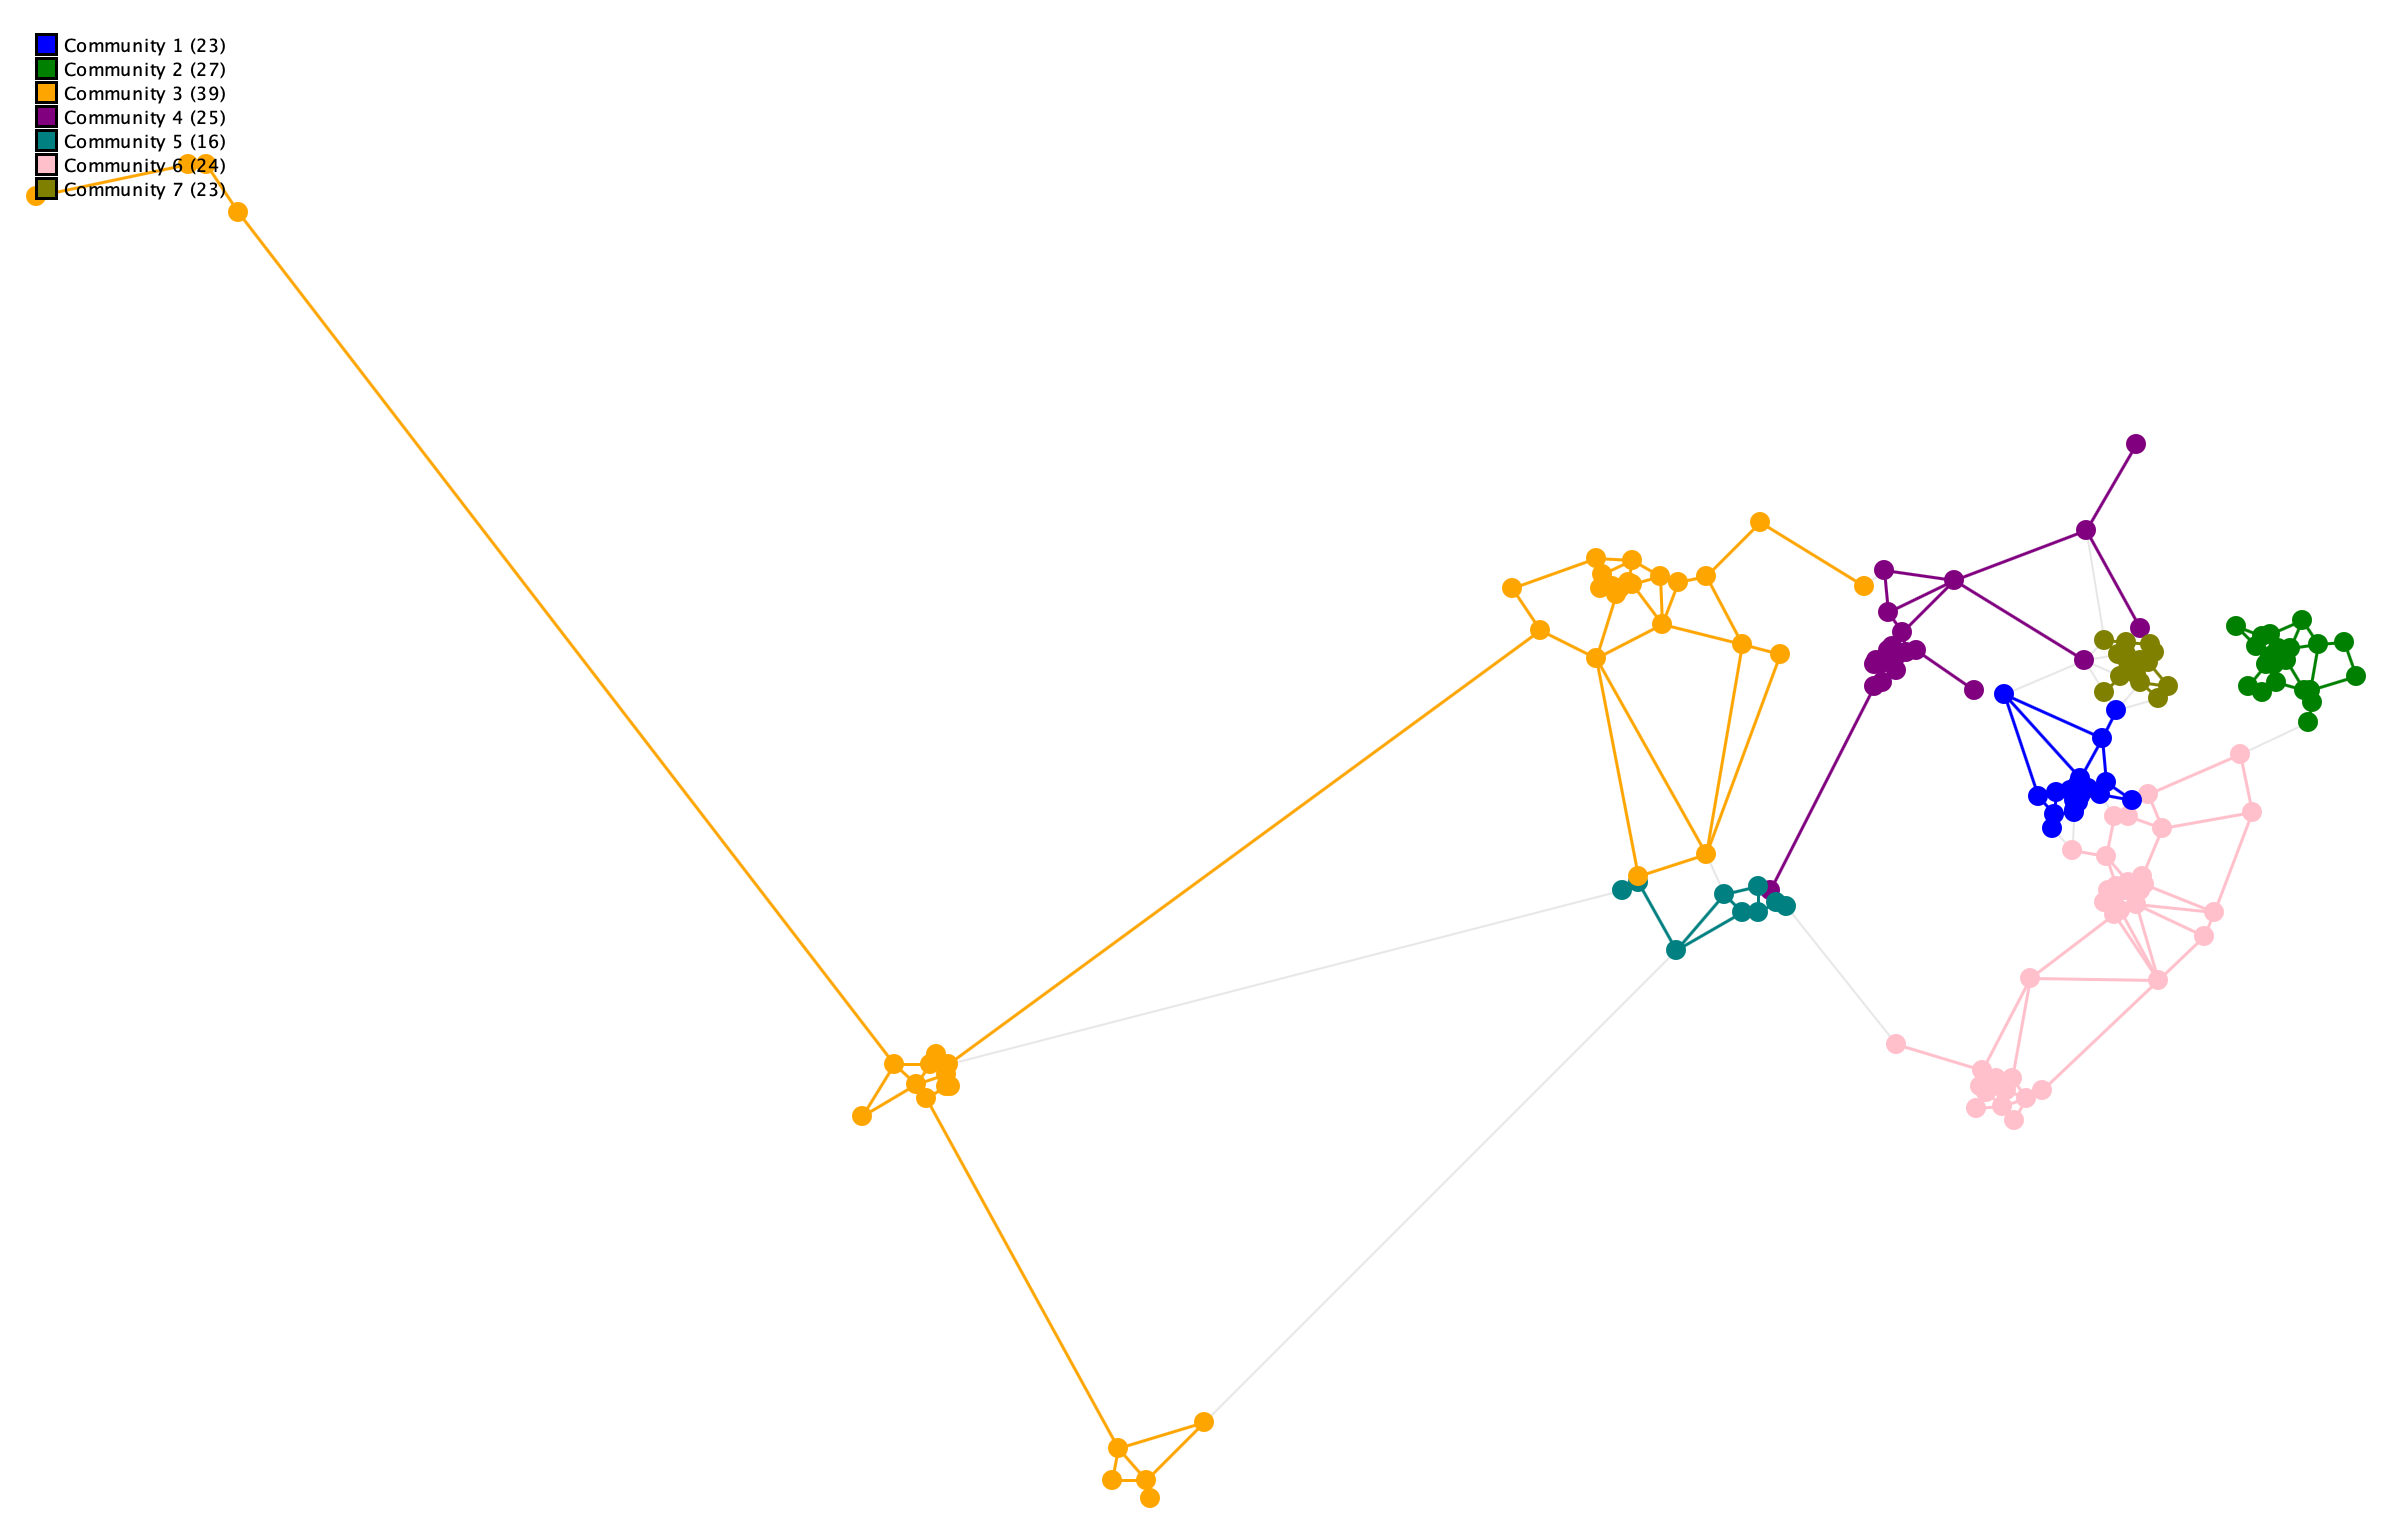
\includegraphics[width=0.5\textwidth]{./img/MVAGC_Gabriel}
\vspace{0.5cm}

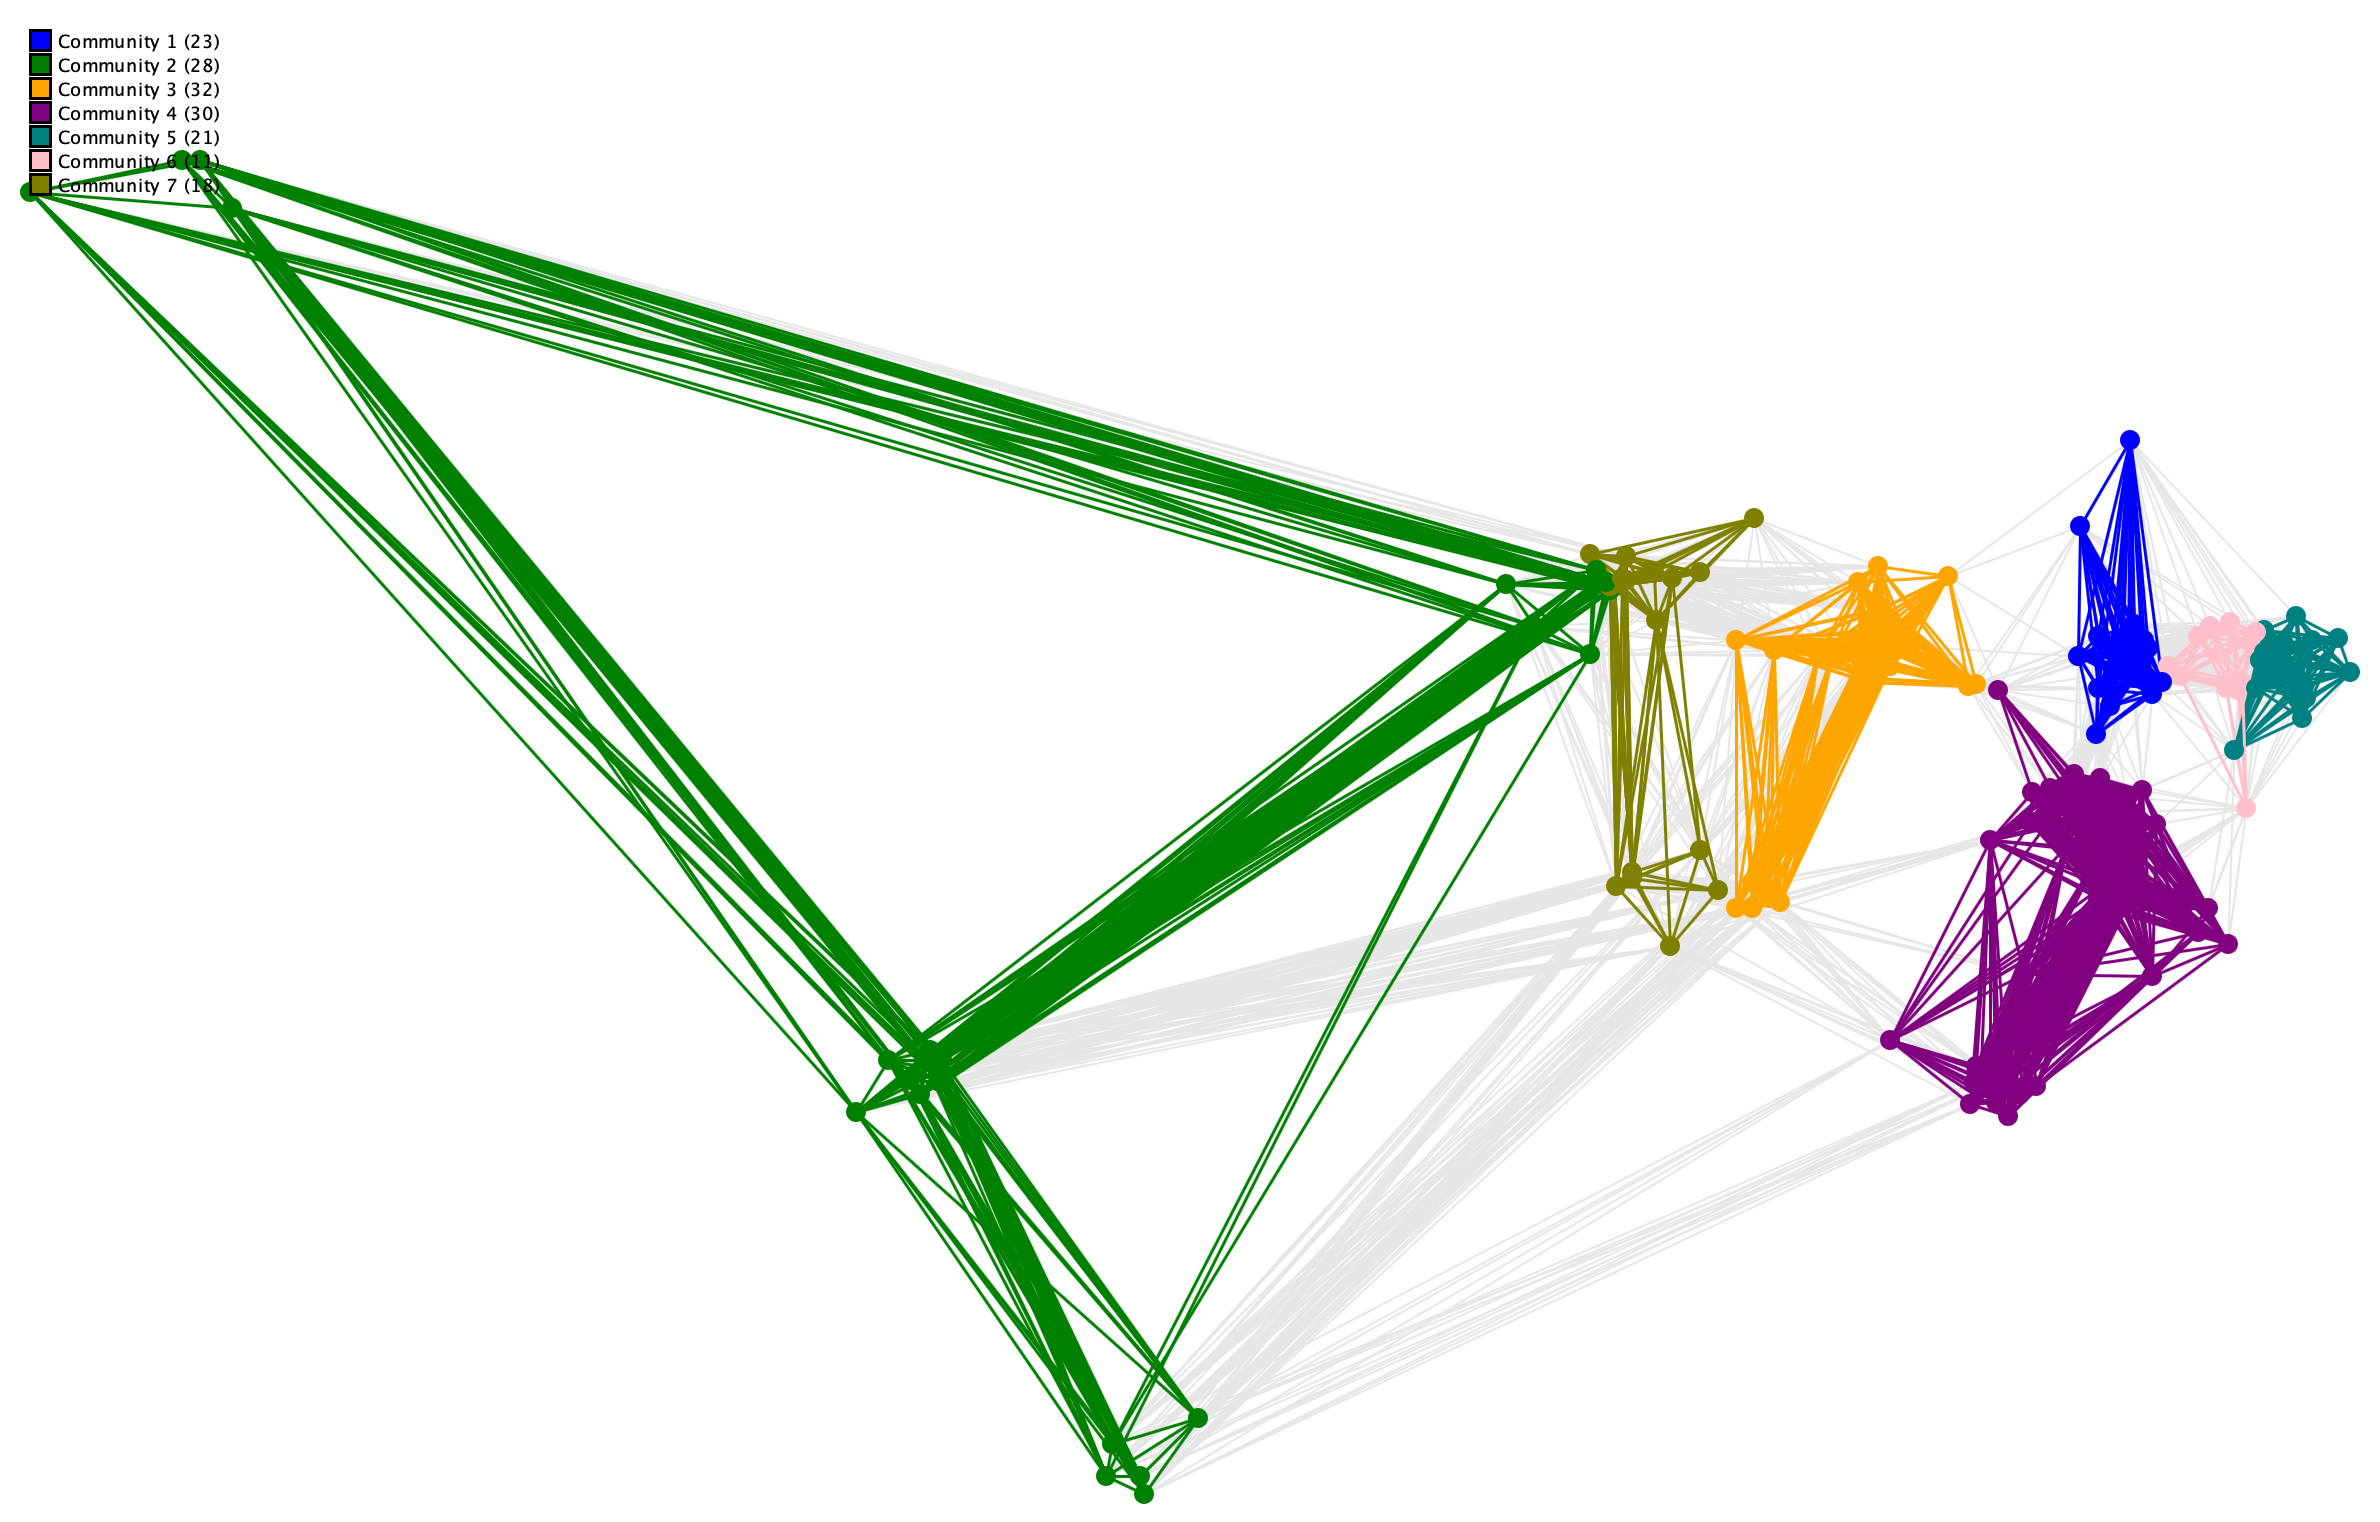
\includegraphics[width=0.5\textwidth]{./img/MVAGC_K}

\caption{MVAGC algorithm applied to different sparse graph representations (top: Delaunay, middle: Gabriel, bottom: K-Nearest) with 200 student locations.}
\label{fig:mvagc_clustering}
\end{figure}

Figure \ref{fig:mvagc_clustering} depicts the clustering patterns of the MVAGC algorithm on various graph representations. On Delaunay triangulation, MVAGC creates numerous small, evenly distributed clusters that follow natural geographic contours; on Gabriel graph, the algorithm generates well-separated clusters with minimal fragmentation; on K-Nearest Neighbors (k=30), MVAGC demonstrates its highest performance, with clusters that naturally adapt to both dense urban areas and sparser suburban regions.

The distinctive clustering pattern produced by our MVAGC implementation shows a higher number of smaller clusters, reflecting the algorithm's anchor-based approach, which captures fine-grained community structures. This visualization demonstrates how MVAGC's multi-view perspective identifies different structural aspects of the transportation network that might be missed by single-view methods.

A notable characteristic of MVAGC is its sensitivity to the underlying graph structure, particularly with the K-Nearest Neighbors graph. This combination produces clusters that closely follow natural residential boundaries and traffic patterns. The method's ability to adapt to local density variations makes it particularly effective for areas with uneven student distribution across Izmir.

The MVAGC approach is well-suited for transportation planning scenarios that prioritize shorter, more efficient routes and have access to a larger number of smaller vehicles.

\subsubsection{Summary of Different Clustering Approaches}
\label{subsubsec:clustering_comparison}

\begin{table}[!hb]
\centering
\begin{tabular}{|l|c|c|c|}
\hline
& \multicolumn{3}{c|}{\textbf{Average Cluster Size}} \\
\hline
\textbf{Algorithm / Graph} & \textbf{Delaunay} & \textbf{Gabriel} & \textbf{KNN} \\
\hline
Spectral & 19.8 & 20.5 & 20.7 \\
\hline
Leiden & 14.5 & 16.4 & 15.8 \\
\hline
MVAGC & 12.7 & 14.5 & 14.3 \\
\hline
\end{tabular}
\caption{Average cluster size for different combinations of graph construction and clustering algorithms}
\label{tab:avg_cluster_size}
\end{table}

\begin{table}[!hb]
\centering
\begin{tabular}{|l|c|c|c|}
\hline
& \multicolumn{3}{c|}{\textbf{Average Route Length (km)}} \\
\hline
\textbf{Algorithm / Graph} & \textbf{Delaunay} & \textbf{Gabriel} & \textbf{KNN} \\
\hline
Spectral & 17.5 & 23.4 & 20.9 \\
\hline
Leiden & 13.7 & 14.0 & 14.1 \\
\hline
MVAGC & 16.6 & 15.8 & 12.4 \\
\hline
\end{tabular}
\caption{Average route length (km) for different combinations of graph construction and clustering algorithms}
\label{tab:avg_route_length}
\end{table}

Tables \ref{tab:avg_cluster_size} and \ref{tab:avg_route_length} summarize the key performance indicators for different clustering algorithms across sparse graph representations. Table \ref{tab:avg_cluster_size} reports the average cluster size in terms of the number of students per route, while Table \ref{tab:avg_route_length} presents the corresponding average route length in kilometers. These metrics illustrate the inherent tendencies of each clustering method and graph combination rather than final performance metrics, which are analyzed in Chapter~\ref{ch:experiments}.

From Table \ref{tab:avg_cluster_size}, MVAGC produces the smallest clusters (12.7--14.5 students), Leiden yields moderate cluster sizes (14.5--16.4 students), and Spectral generates the largest clusters (19.8--20.7 students), reflecting their relative granularity. Considering graph structures, the K-Nearest Neighbors graph tends to increase cluster sizes for Spectral (20.7 students) and decrease them for MVAGC (14.3 students).

Table \ref{tab:avg_route_length} shows that Leiden achieves the shortest average routes (13.7--14.1 km), indicating a balanced trade-off between compactness and connectivity. Spectral clustering on the Gabriel graph results in the longest routes (23.4 km) due to sparser edge connectivity, whereas MVAGC attains its shortest routes on the KNN graph (12.4 km), highlighting the advantage of locally dense connections for route optimization. Overall, the K-Nearest Neighbors representation strikes a favorable balance between cluster cohesion and route efficiency across all algorithms.

\section{The Shortest Path Algorithm for Service Route Determinationn}
\label{sec:shortest_path}

After clustering the student locations into communities that represent potential bus routes, determining the optimal path through each cluster becomes essential for minimizing travel distance, time, and fuel consumption. We implemented Dijkstra's algorithm as the core method for computing optimal routes within each cluster.

This approach leverages the efficiency of Dijkstra's algorithm while addressing the practical challenges of route planning. Figure \ref{fig:route_optimization} illustrates a sample optimized route for a cluster.

\begin{figure}[!htbp]
\centering
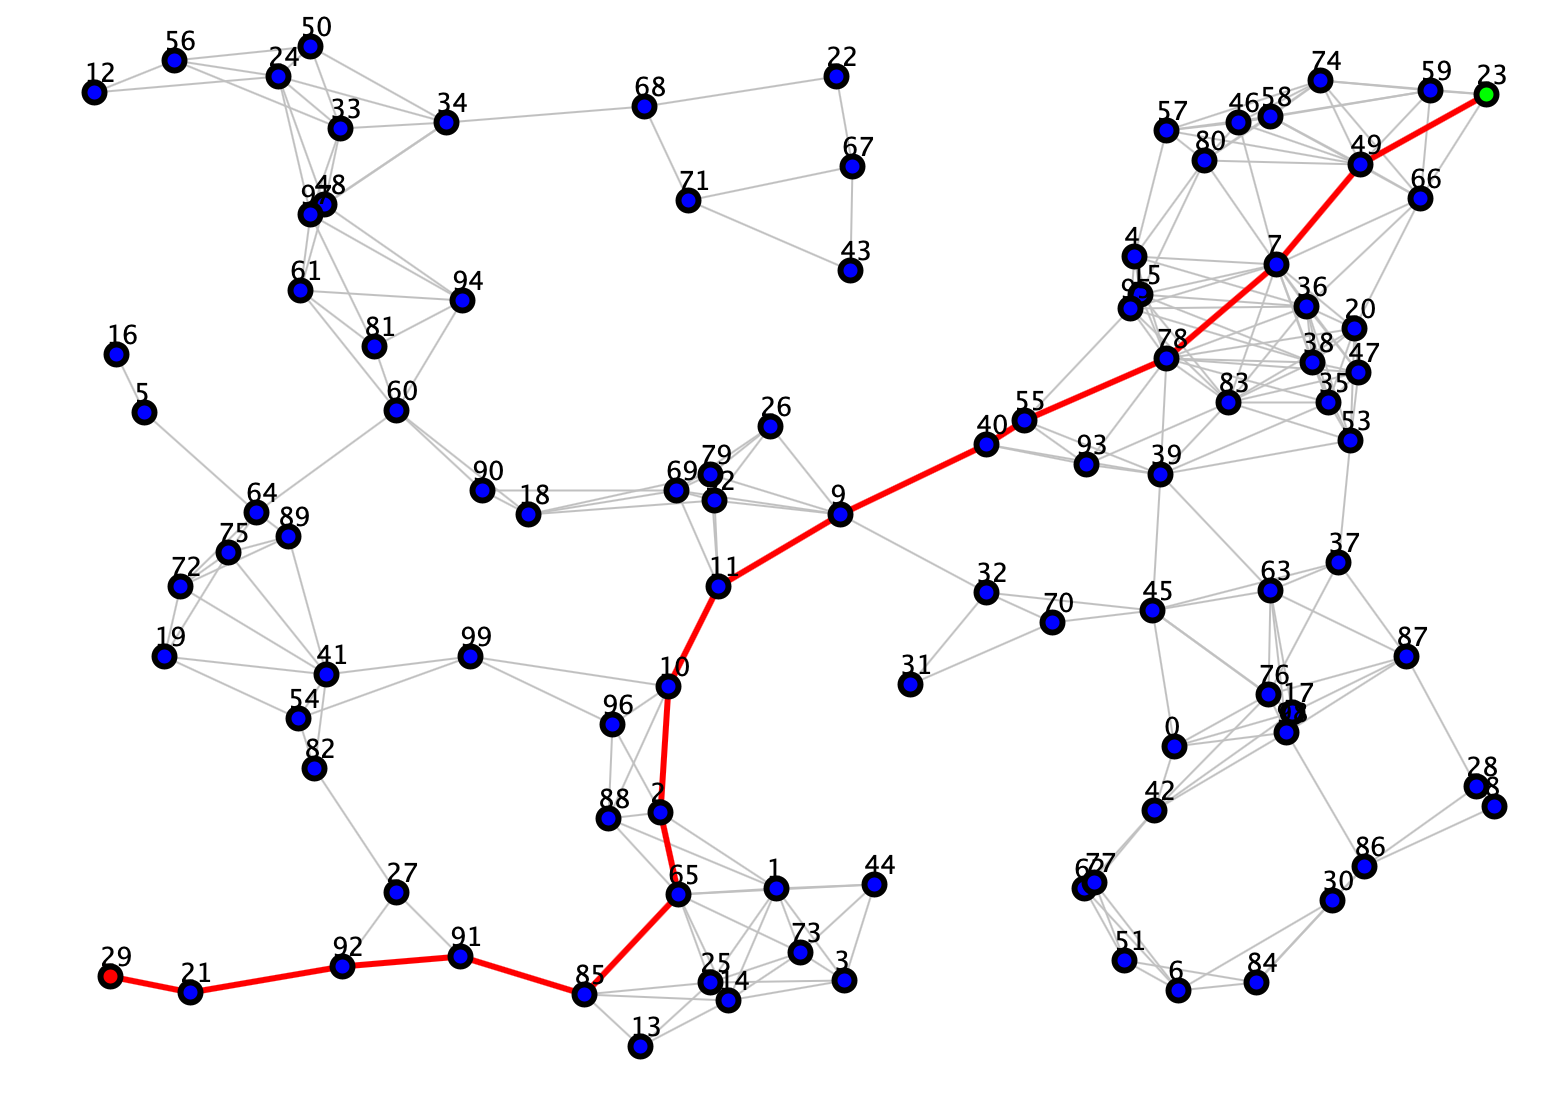
\includegraphics[width=0.8\textwidth]{img/shortest_path}
\caption{Example of an optimized route through a cluster of student locations. The red line represents the shortest path computed using Dijkstra's algorithm.}
\label{fig:route_optimization}
\end{figure}

\section{Robustness for Isolated Vertices of Distant Addresses}
\label{sec:robustness}

To ensure the reliability and validity of the clustering results and subsequent route optimization, it is important to consider the robustness of the approach. This involves assessing how sensitive the outcomes are to variations in the input data or parameters. One crucial step performed prior to clustering was outlier detection, aimed at identifying and potentially removing data points that could disproportionately affect the clustering process and lead to impractical or inefficient routes.

\subsection{KNN Outlier Detection}
\label{subsec:knn_outlier_application}

Before applying the clustering algorithms described in Section~\ref{sec:clustering_graph}, we implemented an outlier detection step using the K-Nearest Neighbor (KNN) distance method (detailed theoretically in Section~\ref{subsec:KNNDistanceOutlier}). The primary goal was to identify student locations from the synthetic dataset that were either unusually isolated. Such points could negatively impact the formation of sensible and efficient transportation clusters.

We extensively tuned the KNN distance algorithm parameters through multiple experimental iterations. After careful analysis, we selected $k=5$ as the optimal number of neighbors for our dataset. This choice balanced computational efficiency with the statistical significance needed to identify genuine outliers. For each student location (node), the average Euclidean distance to its 5 nearest neighbors was calculated. We then computed the mean and standard deviation of these average distances across all nodes in the dataset.

A node was flagged as an outlier if its average 5-NN distance deviated significantly from the overall mean. We conducted a systematic investigation to determine the optimal standard deviation threshold, experimenting with values ranging from 0.5 to 8.0. This parameter tuning process was critical to balance the trade-off between excluding too many students (resulting in reduced service coverage) and including outliers that would significantly increase transportation costs. Specifically, we used a standard deviation threshold of 6.5 for our final implementation. Any node whose average 5-NN distance was more than 6.5 standard deviations away from the mean (either above or below) was marked as an outlier. Nodes identified as outliers were subsequently excluded from the graph representations before the clustering algorithms were executed. This preprocessing step helped to refine the dataset, removing potential noise and improving the quality and practicality of the resulting transportation clusters and routes.

Figure \ref{fig:outlier_cost} illustrates the impact of different standard deviation thresholds on both the number of outliers excluded and the resulting total transportation cost. As the threshold increases, fewer data points are classified as outliers, resulting in more students being included in the routing solution. The analysis reveals that there exists an optimal threshold value that balances the trade-off between inclusivity and cost-efficiency, proving that we could achieve further cost reductions beyond our initial Gabriel+Leiden clustering approach.

\begin{figure}[!htbp]
\centering
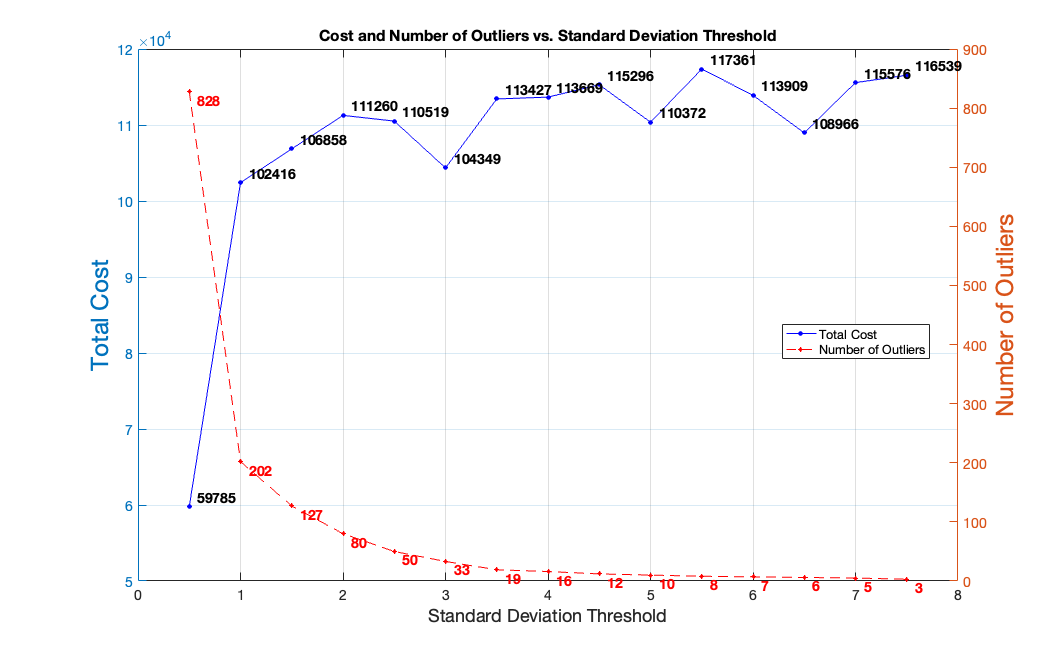
\includegraphics[width=\textwidth]{img/KNN_distance_outlier_cost}
\caption{Cost and Number of Outliers vs. Standard Deviation Threshold. The blue line represents the total transportation cost, while the red dashed line indicates the number of outliers excluded at each threshold level. As the standard deviation threshold increases, fewer outliers are excluded and the cost stabilizes.}
\label{fig:outlier_cost}
\end{figure}

% Commenting out the example algorithm from the template
% \begin{algorithm}
% \begin{algorithmic}[1]
% \STATE generate random number $n \in [l, u]$
% \WHILE{$n \neq 42$}
% \IF{today is Tuesday}
% \STATE print(42)
% \ENDIF
% \ENDWHILE
% \RETURN best solution found so far
% \end{algorithmic}
% \caption{Basic Algorithm($l, u$)}
% \label{alg:example_alg}
% \end{algorithm}



